% =====================================================================
%  Báo cáo bài tập lớn – Nhập môn Học máy (FIT4013)
%  Đề tài 8: Dự đoán sinh viên có nguy cơ bỏ học
%  Biên dịch: pdfLaTeX (Overleaf mặc định) – chạy 2 lần để có mục lục.
% =====================================================================
\documentclass[12pt,a4paper,oneside]{report}

% ---------- Ngôn ngữ và phông chữ ----------
\usepackage[utf8]{inputenc}
\usepackage[T5]{fontenc}
\usepackage[vietnamese]{babel}
\usepackage{lmodern}
\usepackage{icomma}               % dấu phẩy thập phân trong chế độ toán
% Tiếng Việt không ngắt từ giữa âm tiết: tắt gạch nối, cho phép giãn khoảng trắng
\AtBeginDocument{\hyphenpenalty=10000 \exhyphenpenalty=10000}
\setlength{\emergencystretch}{3em}

% ---------- Trình bày trang ----------
\usepackage[left=3cm,right=2cm,top=2.5cm,bottom=2.5cm]{geometry}
\usepackage{setspace}\setstretch{1.25}
\usepackage{indentfirst}
\setlength{\parskip}{4pt}
\usepackage{titlesec}
\titleformat{\chapter}[display]{\bfseries\Large\centering}{\MakeUppercase{\chaptertitlename}\ \thechapter}{6pt}{\LARGE\MakeUppercase}
\titlespacing*{\chapter}{0pt}{-10pt}{18pt}
\titleformat{\section}{\bfseries\large}{\thesection}{0.6em}{}
\titleformat{\subsection}{\bfseries\normalsize}{\thesubsection}{0.6em}{}
\usepackage{fancyhdr}
\pagestyle{fancy}\fancyhf{}
\fancyhead[L]{\small Nhập môn Học máy -- Đề tài 8}
\fancyhead[R]{\small EduRisk}
\fancyfoot[C]{\thepage}
\renewcommand{\headrulewidth}{0.4pt}
\setlength{\headheight}{15pt}
\fancypagestyle{plain}{\fancyhf{}\fancyfoot[C]{\thepage}\renewcommand{\headrulewidth}{0pt}}

% ---------- Bảng, hình, mã ----------
\usepackage{amsmath,amssymb}
\usepackage{graphicx}\graphicspath{{figures/}}
\usepackage{booktabs,tabularx,multirow,array,longtable}
\usepackage{xcolor,colortbl}
\usepackage{caption}\captionsetup{font=small,labelfont=bf}
\usepackage{float}
\usepackage{enumitem}\setlist{itemsep=2pt,topsep=4pt}
\usepackage{listings}
\usepackage{tikz}\usetikzlibrary{positioning,arrows.meta,shapes.geometric,calc,fit}
\usepackage[unicode,hidelinks]{hyperref}

\definecolor{navy}{HTML}{0B2A5B}
\definecolor{accent}{HTML}{F26F21}
\definecolor{codebg}{HTML}{F5F7FB}
\definecolor{best}{HTML}{E6F0FF}

\lstdefinestyle{py}{language=Python,basicstyle=\ttfamily\footnotesize,backgroundcolor=\color{codebg},
  keywordstyle=\color{navy}\bfseries,commentstyle=\color{gray}\itshape,stringstyle=\color{accent!80!black},
  frame=single,rulecolor=\color{gray!40},breaklines=true,columns=fullflexible,showstringspaces=false,
  numbers=left,numberstyle=\tiny\color{gray},xleftmargin=1.5em,framexleftmargin=1.5em}
\lstset{style=py}

\addto\captionsvietnamese{%
  \renewcommand{\contentsname}{Mục lục}
  \renewcommand{\listfigurename}{Danh mục hình}
  \renewcommand{\listtablename}{Danh mục bảng}
  \renewcommand{\bibname}{Tài liệu tham khảo}
  \renewcommand{\figurename}{Hình}
  \renewcommand{\tablename}{Bảng}
  \renewcommand{\chaptername}{Chương}
  \renewcommand{\appendixname}{Phụ lục}
  \renewcommand{\lstlistingname}{Đoạn mã}}

\newcommand{\code}[1]{\texttt{#1}}
\newcommand{\fone}{Macro-F1}

% ---------- Thông tin nhóm: SỬA TẠI ĐÂY ----------
\newcommand{\memberA}{Nguyễn Đăng Quang & 1871020481 & Nhóm trưởng; EDA, tiền xử lý}
\newcommand{\memberB}{Nguyễn Thị Tuyết & 1871020644 & Mô hình, thí nghiệm, đánh giá}
\newcommand{\memberC}{Đỗ Trung Kiên & 1871020344 & Ứng dụng web, báo cáo}
\newcommand{\className}{(CNTT 18-09)}
\newcommand{\repoURL}{\url{https://github.com/itzryuka/FIT4013-EduRisk}}

\begin{document}

% =====================================================================
%  TRANG BÌA
% =====================================================================
\pagenumbering{alph}
\begin{titlepage}
\begin{center}
\setstretch{1.15}
{\large\bfseries BỘ GIÁO DỤC VÀ ĐÀO TẠO}\\[2pt]
{\large\bfseries TRƯỜNG ĐẠI HỌC ĐẠI NAM}\\[2pt]
{\large\bfseries KHOA CÔNG NGHỆ THÔNG TIN}\\[4pt]
\rule{0.45\textwidth}{0.8pt}\\[1.2cm]
\IfFileExists{figures/logo.png}{
\includegraphics[height=3.6cm]{logo.png}}{\vspace{3.6cm}}\\[1.2cm]
{\Large\bfseries BÁO CÁO BÀI TẬP LỚN}\\[6pt]
{\large HỌC PHẦN: NHẬP MÔN HỌC MÁY (FIT4013)}\\[1.2cm]
{\color{navy}\LARGE\bfseries ĐỀ TÀI 8: DỰ ĐOÁN SINH VIÊN\\[4pt] CÓ NGUY CƠ BỎ HỌC}\\[6pt]
{\large Hệ thống cảnh báo sớm EduRisk}\\[1.4cm]
\begin{tabular}{rl}
Giảng viên hướng dẫn: & ThS. Lê Thị Thùy Trang\\
Lớp: & \className
\end{tabular}\\[0.6cm]
{\bfseries Nhóm sinh viên thực hiện}\\[4pt]
\begin{tabular}{llp{6cm}}
\toprule
\textbf{Họ và tên} & \textbf{MSSV} & \textbf{Nhiệm vụ chính}\\
\midrule
\memberA\\ \memberB\\ \memberC\\
\bottomrule
\end{tabular}
\vfill
{\large Hà Nội, tháng 11 năm 2026}
\end{center}
\end{titlepage}

\pagenumbering{roman}
\chapter*{Tóm tắt}
\addcontentsline{toc}{chapter}{Tóm tắt}
Báo cáo trình bày quá trình xây dựng một hệ thống học máy dự đoán kết cục học tập của sinh viên đại học thành ba lớp:
\emph{Bỏ học} (Dropout), \emph{Còn đang học} (Enrolled) và \emph{Tốt nghiệp} (Graduate). Nhóm sử dụng bộ dữ liệu công khai
\emph{Predict Students' Dropout and Academic Success} (UCI \#697) gồm 4.424 sinh viên và 36 đặc trưng.

Điểm khác biệt chính của bài làm là xét bài toán theo \textbf{ba thời điểm dự đoán} (lúc nhập học, sau học kỳ 1, sau năm thứ nhất)
để tránh dùng thông tin ``tương lai''. Nhóm so sánh ba thuật toán (K-Nearest Neighbors, Gaussian Naive Bayes, Decision Tree)
trên hai luồng tiền xử lý (cơ bản và có kỹ thuật đặc trưng), với tham số mặc định và tham số tinh chỉnh bằng \code{GridSearchCV}.
Tổng cộng 39 cấu hình được đánh giá. Mô hình được chọn theo \fone{} kiểm định chéo, không theo tập kiểm tra.

Trên tập kiểm tra độc lập (885 sinh viên), mô hình Decision Tree đạt \fone{} 0,531 lúc nhập học, 0,634 sau học kỳ 1 và
0,673 sau năm thứ nhất, so với 0,222 của mốc so sánh luôn đoán lớp đông nhất. Kỹ thuật đặc trưng (Luồng B) giúp K-NN và
Naive Bayes tăng 0,04--0,07 điểm \fone{}. Lớp \emph{Còn đang học} là lớp khó phân biệt nhất. Mô hình được triển khai thành
ứng dụng web Flask có chức năng dự đoán từng sinh viên, dự đoán theo danh sách và giải thích lý do dự đoán.

\textbf{Từ khóa:} dự đoán bỏ học, phân loại đa lớp, dữ liệu mất cân bằng, K-NN, Naive Bayes, cây quyết định, scikit-learn.

\tableofcontents
\listoffigures
\listoftables
\clearpage
\pagenumbering{arabic}

% =====================================================================
\chapter{Đặt vấn đề và phân tích yêu cầu}
% =====================================================================
\section{Bối cảnh}
Bỏ học là vấn đề gây tổn thất cho cả sinh viên, gia đình và nhà trường: sinh viên mất thời gian và chi phí,
nhà trường mất nguồn lực đào tạo và bị ảnh hưởng tới các chỉ số kiểm định. Phần lớn trường hợp bỏ học có dấu hiệu từ sớm
như nợ học phí, trượt nhiều môn ở năm đầu hay không đăng ký học phần. Nếu phát hiện kịp thời, phòng công tác sinh viên và
cố vấn học tập có thể can thiệp bằng tư vấn, hỗ trợ học bổng hoặc kèm cặp học tập.

Khó khăn là số lượng sinh viên lớn, cán bộ không thể theo dõi từng người. Học máy có thể giúp \textbf{xếp hạng sinh viên theo
mức nguy cơ} để nhà trường ưu tiên nguồn lực hỗ trợ cho những người cần nhất.

\section{Mục tiêu và phạm vi}
\textbf{Bài toán:} cho thông tin của một sinh viên, dự đoán sinh viên đó thuộc lớp nào trong ba lớp
\emph{Bỏ học}, \emph{Còn đang học} (chưa tốt nghiệp sau thời gian chuẩn) hoặc \emph{Tốt nghiệp}.
Đây là bài toán \textbf{phân loại có giám sát, đa lớp}.

\textbf{Mục tiêu cụ thể:}
\begin{enumerate}
  \item Phân tích dữ liệu, xác định các yếu tố liên quan tới bỏ học.
  \item Xây dựng quy trình học máy có thể tái lập, không rò rỉ dữ liệu.
  \item So sánh ba thuật toán K-NN, Naive Bayes, Decision Tree và hai cách tiền xử lý; có mốc so sánh (baseline) rõ ràng.
  \item Đánh giá mức độ chính xác ở từng thời điểm dự đoán, từ đó trả lời câu hỏi ``có thể cảnh báo sớm đến mức nào''.
  \item Phân tích lỗi và triển khai mô hình thành ứng dụng web có giải thích.
\end{enumerate}

\textbf{Tiêu chí đánh giá chính:} \fone{} (trung bình F1 của ba lớp), vì dữ liệu mất cân bằng và lớp thiểu số
\emph{Bỏ học}, \emph{Còn đang học} quan trọng không kém lớp đông nhất. Accuracy và ROC-AUC được báo cáo bổ sung.

\section{Mô tả dữ liệu}
Bộ dữ liệu do Realinho và cộng sự công bố năm 2022 \cite{realinho2022}, lưu trữ tại UCI Machine Learning Repository \cite{uci697}
theo giấy phép CC BY 4.0. Dữ liệu thu thập tại Học viện Bách khoa Portalegre (Bồ Đào Nha) cho các khóa nhập học từ 2008--2009
đến 2018--2019, thuộc 17 ngành đào tạo bậc cử nhân.

\begin{itemize}
  \item \textbf{Kích thước:} 4.424 dòng (mỗi dòng là một sinh viên), 36 đặc trưng và 1 cột nhãn \code{Target}.
  \item \textbf{Định dạng:} tệp CSV phân tách bằng dấu chấm phẩy; các biến phân loại đã được mã hóa thành số nguyên theo bảng mã của bài báo gốc.
\end{itemize}

Bảng~\ref{tab:groups} chia 36 đặc trưng thành các nhóm theo ý nghĩa và theo thời điểm có thông tin.
\begin{table}[H]
\centering\small
\caption{Các nhóm đặc trưng trong bộ dữ liệu}\label{tab:groups}
\begin{tabularx}{\textwidth}{@{}p{3.6cm}cX@{}}
\toprule
\textbf{Nhóm} & \textbf{Số cột} & \textbf{Ví dụ}\\
\midrule
Nhân khẩu học & 6 & Tình trạng hôn nhân, quốc tịch, giới tính, tuổi nhập học, sinh viên quốc tế, ở xa nhà\\
Tuyển sinh & 6 & Phương thức xét tuyển, thứ tự nguyện vọng, ngành học, học ca ngày/tối, bằng cấp trước, điểm bằng cấp trước, điểm xét tuyển\\
Gia đình & 4 & Trình độ học vấn và nghề nghiệp của cha, mẹ\\
Tài chính, hỗ trợ & 4 & Nợ, đóng học phí đúng hạn, học bổng, nhu cầu giáo dục đặc biệt\\
Kinh tế vĩ mô & 3 & Tỉ lệ thất nghiệp, lạm phát, GDP năm nhập học\\
Học kỳ 1 & 6 & Số học phần được miễn, đăng ký, số lần đánh giá, số học phần đạt, điểm trung bình, số học phần không dự thi\\
Học kỳ 2 & 6 & Tương tự học kỳ 1\\
\midrule
Nhãn & 1 & \code{Target}: Dropout / Enrolled / Graduate\\
\bottomrule
\end{tabularx}
\end{table}

Theo kiểu dữ liệu, có 9 biến \textbf{danh nghĩa} (mã ngành, nghề nghiệp\dots{} số mã không mang ý nghĩa thứ tự),
8 biến \textbf{nhị phân} và 19 biến \textbf{số}. Cách phân loại này quyết định cách mã hóa ở Chương~\ref{ch:design}.

\section{Phân tích khám phá dữ liệu (EDA)}
\subsection{Phân phối nhãn}
\begin{figure}[H]
\centering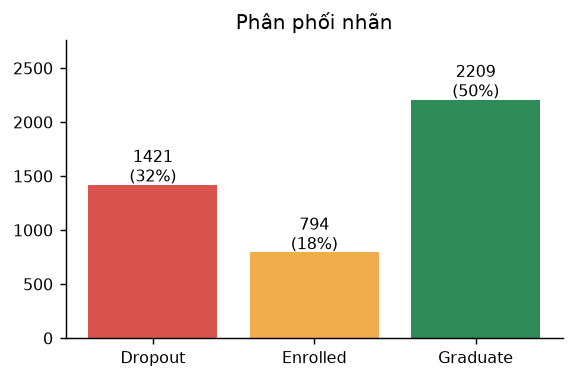
\includegraphics[width=0.55\textwidth]{eda_target_distribution.png}
\caption{Phân phối ba lớp của biến mục tiêu}\label{fig:target}
\end{figure}
Dữ liệu \textbf{mất cân bằng}: Tốt nghiệp 49,9\% (2.209), Bỏ học 32,1\% (1.421), Còn đang học 17,9\% (794).
Hệ quả: (i) một mô hình ``luôn đoán Tốt nghiệp'' đã đạt accuracy gần 50\% nên accuracy không phải thước đo tốt;
(ii) cần chia dữ liệu phân tầng (stratified) để tỉ lệ lớp ở tập huấn luyện và tập kiểm tra như nhau;
(iii) nên thử trọng số lớp (\code{class\_weight}) cho các thuật toán hỗ trợ.

\subsection{Chất lượng dữ liệu}
\begin{itemize}
  \item \textbf{Không có giá trị thiếu} và \textbf{không có dòng trùng lặp}.
  \item \textbf{Cột gần như hằng số:} \code{Educational special needs} (98,8\% cùng một giá trị), \code{International} và
        \code{Nacionality} (97,5\%). Các cột này gần như không mang thông tin nhưng làm tăng số chiều sau One-Hot.
  \item \textbf{``Giá trị thiếu trá hình'':} 180 sinh viên đăng ký 0 học phần ở cả hai học kỳ, nên điểm trung bình bằng 0.
        Số 0 ở đây nghĩa là ``không có điểm'' chứ không phải ``điểm kém'' (75 người trong nhóm này vẫn tốt nghiệp, có thể nhờ được miễn học phần).
  \item \textbf{Lệch phân phối:} tuổi nhập học lệch phải mạnh (trung vị 20, lớn nhất 70, hệ số lệch 2,05).
  \item \textbf{Mã hiếm:} nhiều biến danh nghĩa có những mã chỉ xuất hiện vài lần (ví dụ nghề nghiệp của cha có 46 mã khác nhau).
  \item Tên một cột trong tệp gốc có ký tự tab ở cuối; chương trình loại bỏ khoảng trắng thừa khi đọc dữ liệu.
\end{itemize}

\subsection{Quan hệ giữa đặc trưng và nhãn}
\begin{figure}[H]
\centering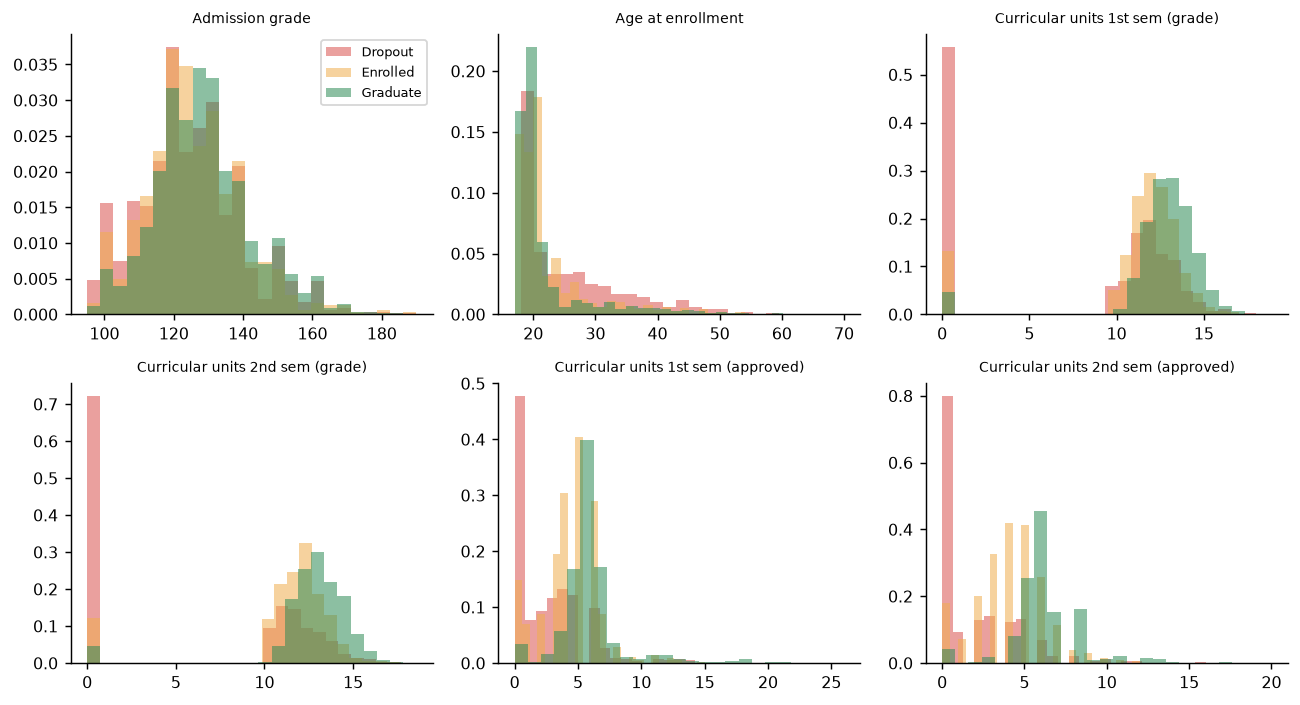
\includegraphics[width=\textwidth]{eda_histograms_by_target.png}
\caption{Phân phối một số đặc trưng số theo từng lớp}\label{fig:hist}
\end{figure}
\begin{figure}[H]
\centering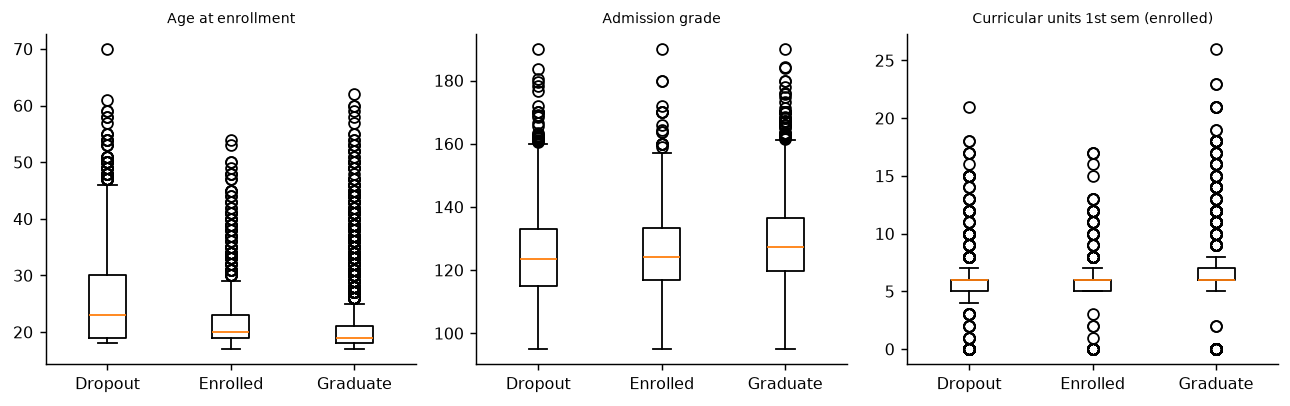
\includegraphics[width=\textwidth]{eda_boxplots.png}
\caption{Biểu đồ hộp của các đặc trưng chính theo lớp}\label{fig:box}
\end{figure}

Các quan sát quan trọng:
\begin{itemize}
  \item \textbf{Kết quả học tập là tín hiệu mạnh nhất.} Số học phần đạt ở học kỳ 2 trung bình là 1,94 ở nhóm Bỏ học,
        4,06 ở nhóm Còn đang học và 6,18 ở nhóm Tốt nghiệp.
  \item \textbf{Học phí:} trong số sinh viên \emph{không} đóng học phí đúng hạn, 86,6\% bỏ học; ở nhóm đóng đúng hạn tỉ lệ này là 24,7\%.
  \item \textbf{Học bổng:} sinh viên có học bổng có tỉ lệ bỏ học 12,2\%, so với 38,7\% ở nhóm không có học bổng.
  \item \textbf{Tuổi:} nhóm Bỏ học có tuổi nhập học trung bình 26,1, cao hơn nhóm Tốt nghiệp (21,8); người lớn tuổi thường vừa học vừa làm.
  \item \textbf{Lớp Còn đang học nằm giữa} hai lớp còn lại trên hầu hết các đặc trưng, nên dự kiến sẽ khó phân biệt nhất.
\end{itemize}

\begin{figure}[H]
\centering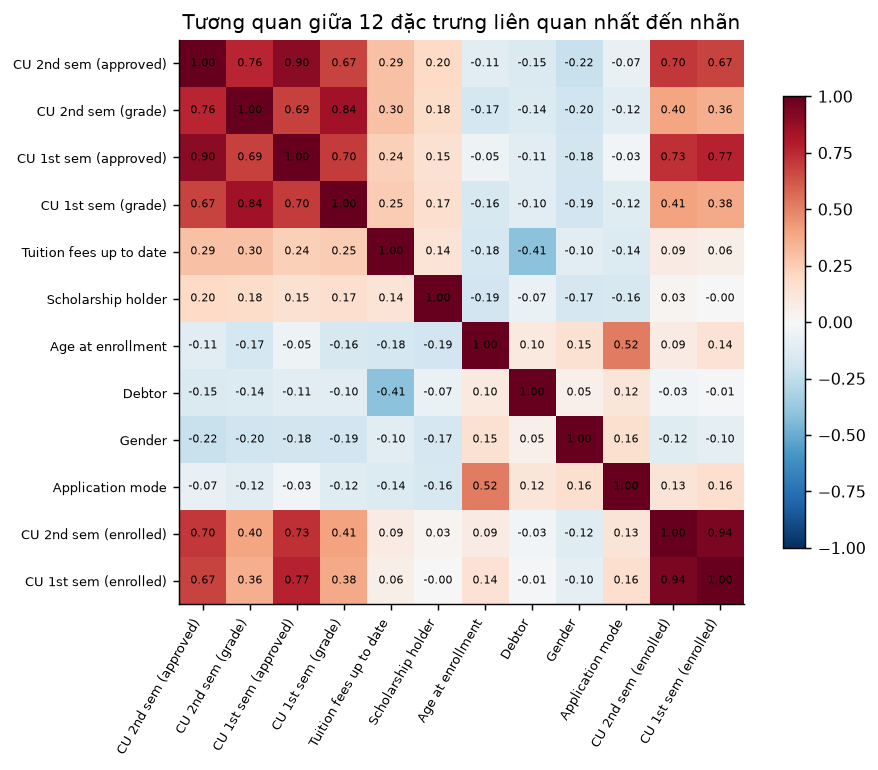
\includegraphics[width=0.72\textwidth]{eda_correlation.png}
\caption{Ma trận tương quan của 12 đặc trưng liên quan nhất đến nhãn}\label{fig:corr}
\end{figure}
Hình~\ref{fig:corr} cho thấy các cột của cùng một học kỳ tương quan rất cao với nhau (số học phần đăng ký, đạt, điểm), và
học kỳ 1 tương quan cao với học kỳ 2. Điều này vi phạm giả định độc lập có điều kiện của Naive Bayes và là lý do nhóm thử
thêm các đặc trưng dạng tỉ lệ ở Luồng B.

\section{Nhận xét rút ra cho thiết kế}
\begin{enumerate}
  \item Dữ liệu mất cân bằng $\Rightarrow$ dùng \fone{}, chia phân tầng, thử \code{class\_weight}.
  \item Biến danh nghĩa mã hóa bằng số $\Rightarrow$ phải One-Hot, không được dùng trực tiếp như số (đặc biệt với K-NN).
  \item Các đặc trưng có thang đo khác nhau (điểm 0--200, tuổi 17--70, số môn 0--26) $\Rightarrow$ chuẩn hóa cho K-NN.
  \item Kết quả học kỳ mạnh nhưng chỉ có \emph{sau} khi học $\Rightarrow$ phải tách kịch bản theo thời điểm dự đoán.
  \item Cột gần hằng số, mã hiếm, số 0 trá hình, tuổi lệch $\Rightarrow$ cơ sở cho Luồng B.
\end{enumerate}

% =====================================================================
\chapter{Thiết kế giải pháp và quy trình học máy}\label{ch:design}
% =====================================================================
\section{Quy trình tổng thể}
\begin{figure}[H]
\centering
\begin{tikzpicture}[node distance=0.45cm and 0.5cm, font=\small,
  box/.style={draw=navy, fill=navy!6, rounded corners=3pt, align=center, minimum height=1cm, text width=2.6cm},
  hl/.style={box, draw=accent, fill=accent!10},
  arr/.style={-{Stealth[length=2.2mm]}, thick, navy}]
\node[box] (raw) {Dữ liệu thô\\ \code{data.csv}};
\node[box, right=of raw] (split) {Chia train/test\\ 80/20 phân tầng};
\node[box, right=of split] (scen) {Chọn cột theo\\ kịch bản};
\node[box, right=of scen] (fe) {Feature-\\Engineer (A/B)};
\node[box, below=1.1cm of fe] (prep) {One-Hot +\\ StandardScaler};
\node[box, left=of prep] (model) {K-NN / NB / DT};
\node[box, left=of model] (gs) {GridSearchCV\\ 5-fold, \fone{}};
\node[hl, left=of gs] (sel) {Chọn theo CV,\\ đánh giá trên test};
\draw[arr] (raw) -- (split); \draw[arr] (split) -- (scen); \draw[arr] (scen) -- (fe);
\draw[arr] (fe) -- (prep); \draw[arr] (prep) -- (model); \draw[arr] (model) -- (gs); \draw[arr] (gs) -- (sel);
\node[draw=accent, dashed, rounded corners, fit=(fe)(prep)(model), inner sep=7pt] (pl) {};
\node[accent, font=\footnotesize, anchor=north west] at (pl.south west) {Pipeline của scikit-learn};
\node[below=0.5cm of sel, box, text width=3cm] (app) {Lưu \code{.joblib}\\ $\rightarrow$ ứng dụng web};
\draw[arr] (sel) -- (app);
\end{tikzpicture}
\caption{Quy trình từ dữ liệu thô đến mô hình triển khai}\label{fig:pipeline}
\end{figure}
Ba bước \code{FeatureEngineer}, tiền xử lý và mô hình được ghép vào một đối tượng \code{Pipeline}. Khi gọi \code{fit},
mọi tham số học từ dữ liệu (danh sách mã One-Hot, trung bình và độ lệch chuẩn của StandardScaler) chỉ được tính trên phần
dữ liệu huấn luyện của mỗi lần kiểm định chéo. Mô hình đã lưu chứa toàn bộ pipeline nên ứng dụng web chỉ cần đưa vào
dữ liệu gốc.

\section{Ba kịch bản theo thời điểm dự đoán}
Nếu dùng cả 36 cột để dự đoán cho một sinh viên vừa nhập học thì mô hình đang dùng dữ liệu chưa tồn tại (điểm học kỳ 2).
Đây là \textbf{rò rỉ theo thời gian}: kết quả đánh giá sẽ đẹp nhưng không dùng được khi cần cảnh báo sớm. Nhóm định nghĩa
ba kịch bản (Bảng~\ref{tab:scen}) và huấn luyện mô hình riêng cho từng kịch bản.

\begin{table}[H]
\centering\small
\caption{Ba kịch bản dự đoán}\label{tab:scen}
\begin{tabularx}{\textwidth}{@{}llcX@{}}
\toprule
\textbf{Mã} & \textbf{Thời điểm} & \textbf{Số cột} & \textbf{Thông tin sử dụng}\\
\midrule
\code{admission} & Lúc nhập học & 24 & Nhân khẩu học, tuyển sinh, gia đình, tài chính, kinh tế vĩ mô\\
\code{sem1} & Sau học kỳ 1 & 30 & Như trên + 6 cột kết quả học kỳ 1\\
\code{full} & Sau năm thứ nhất & 36 & Toàn bộ, gồm cả học kỳ 2\\
\bottomrule
\end{tabularx}
\end{table}
\textbf{Giả định:} thông tin tài chính (nợ, học phí, học bổng) được xem là có từ đầu khóa. Trong thực tế trạng thái học phí
có thể thay đổi theo học kỳ; đây là một hạn chế được nêu ở Chương~\ref{ch:discuss}.

\section{Làm sạch, mã hóa và chuẩn hóa}
Nhóm xây dựng hai luồng tiền xử lý để đo xem kỹ thuật đặc trưng có thực sự giúp ích hay không.

\textbf{Luồng A -- cơ bản.} Giữ nguyên các cột của kịch bản. Biến danh nghĩa được One-Hot đầy đủ
(\code{handle\_unknown="ignore"} để mã lạ ở tập kiểm tra không gây lỗi). Biến số và nhị phân được chuẩn hóa bằng
\code{StandardScaler}.

\textbf{Luồng B -- cải tiến.} Mỗi thay đổi xuất phát từ một quan sát ở phần EDA (Bảng~\ref{tab:flowb}).
\begin{table}[H]
\centering\small
\caption{Các bước bổ sung của Luồng B và lý do}\label{tab:flowb}
\begin{tabularx}{\textwidth}{@{}p{5.2cm}X@{}}
\toprule
\textbf{Bước} & \textbf{Lý do}\\
\midrule
Bỏ 3 cột gần hằng số & Gần như không có thông tin, chỉ thêm chiều nhiễu cho K-NN\\
Gộp mã xuất hiện $<1\%$ (\code{min\_frequency=0.01}) & Giảm số cột One-Hot; mã hiếm khiến khoảng cách K-NN bị nhiễu và ước lượng xác suất của NB không ổn định\\
$\log(1+\text{tuổi})$ & Giảm lệch phải, giúp giả định phân phối chuẩn của Gaussian NB hợp lý hơn\\
\code{s1/s2\_approval\_rate} = đạt / đăng ký & Chuẩn hóa theo khối lượng học: đạt 5/5 khác hẳn đạt 5/10\\
\code{s1/s2\_eval\_success} = đạt / số lần đánh giá & Phản ánh hiệu quả thi cử\\
\code{s1/s2\_no\_enrolment} = [đăng ký = 0] & Tách ``số 0 trá hình'' thành một cờ riêng\\
\code{grade\_trend} = điểm HK2 $-$ điểm HK1 & Xu hướng tiến bộ hay sa sút (chỉ có ở kịch bản \code{full})\\
\code{approved\_total} = đạt HK1 + đạt HK2 & Tổng khối lượng tích lũy năm 1\\
\bottomrule
\end{tabularx}
\end{table}
Các phép biến đổi trên là phép tính trên từng dòng, không học tham số từ dữ liệu, nên không gây rò rỉ. Phép chia an toàn
trả về 0 khi mẫu số bằng 0.

\section{Chia dữ liệu và hạn chế rò rỉ dữ liệu}
\begin{itemize}
  \item Chia \textbf{80\% huấn luyện (3.539)} và \textbf{20\% kiểm tra (885)} bằng \code{train\_test\_split} với
        \code{stratify=y}, \code{random\_state=42}. Tập kiểm tra được giữ riêng, chỉ dùng một lần để báo cáo.
  \item Việc chọn siêu tham số dùng \textbf{kiểm định chéo phân tầng 5 phần} chỉ trên tập huấn luyện (lớp \code{StratifiedKFold}, có xáo trộn).
  \item Mọi bước học tham số nằm trong \code{Pipeline} $\Rightarrow$ không có thông tin của phần kiểm định lọt vào lúc huấn luyện.
  \item Rò rỉ theo thời gian được xử lý bằng ba kịch bản.
  \item Mô hình triển khai được chọn theo điểm CV, không theo điểm trên tập kiểm tra.
\end{itemize}

\section{Thuật toán và lý do lựa chọn}
\begin{description}
  \item[K-Nearest Neighbors (K-NN)] \cite{cover1967} phân loại một mẫu theo đa số trong $k$ láng giềng gần nhất.
        Không giả định về phân phối dữ liệu, dễ giải thích bằng ví dụ (``sinh viên này giống những sinh viên nào''). Nhược điểm:
        nhạy với thang đo và với số chiều, nên phụ thuộc mạnh vào tiền xử lý. Tham số tinh chỉnh: $k$, trọng số
        (\code{uniform}/\code{distance}), khoảng cách Manhattan ($p=1$) hay Euclid ($p=2$).
  \item[Gaussian Naive Bayes] áp dụng định lý Bayes với giả định các đặc trưng độc lập khi biết lớp và mỗi đặc trưng có phân phối chuẩn.
        Huấn luyện rất nhanh, cho xác suất, là mốc so sánh tốt cho mô hình xác suất đơn giản. Tham số \code{var\_smoothing}
        cộng thêm một lượng vào phương sai để tránh chia cho số rất nhỏ.
  \item[Decision Tree] \cite{breiman1984} chia dữ liệu bằng các câu hỏi dạng ``đặc trưng $\le$ ngưỡng''. Không cần chuẩn hóa,
        xử lý được quan hệ phi tuyến và tương tác, và đặc biệt \textbf{giải thích được bằng luật}, phù hợp khi kết quả cần trình bày cho
        cán bộ quản lý. Tham số: độ sâu tối đa, số mẫu tối thiểu ở lá, tiêu chí \code{gini}/\code{entropy}, trọng số lớp.
\end{description}
Ba thuật toán đại diện cho ba cách tiếp cận khác nhau (dựa trên khoảng cách, dựa trên xác suất, dựa trên luật), nên việc so
sánh giúp hiểu đặc điểm của dữ liệu chứ không chỉ chọn ra mô hình có điểm cao nhất.

\section{Tinh chỉnh siêu tham số}
\begin{table}[H]
\centering\small
\caption{Không gian tìm kiếm của GridSearchCV}\label{tab:grid}
\begin{tabularx}{\textwidth}{@{}lXr@{}}
\toprule
\textbf{Thuật toán} & \textbf{Lưới tham số} & \textbf{Số tổ hợp}\\
\midrule
K-NN & $k \in \{3;\ 5;\ 7;\ 11;\ 15;\ 21;\ 31;\ 45\}$; weights $\in$ \{uniform; distance\}; $p \in \{1;\ 2\}$ & 32\\
Gaussian NB & var\_smoothing $\in \{10^{-11};\ 10^{-10};\ \dots;\ 10^{-1};\ 1\}$ & 12\\
Decision Tree & max\_depth $\in \{3;\ 4;\ 5;\ 6;\ 8;\ 10;\ \text{None}\}$; min\_samples\_leaf $\in \{1;\ 5;\ 10;\ 20;\ 40;\ 80\}$; criterion $\in$ \{gini; entropy\}; class\_weight $\in$ \{None; balanced\} & 168\\
\bottomrule
\end{tabularx}
\end{table}
Tiêu chí chọn là \fone{} trung bình trên 5 phần. Với mỗi kịch bản, cấu hình có CV cao nhất trong 6 cấu hình đã tinh chỉnh
(3 thuật toán $\times$ 2 luồng) được lưu làm mô hình triển khai.

% =====================================================================
\chapter{Phân tích mã nguồn và chức năng}
% =====================================================================
\section{Cấu trúc chương trình}
Mã nguồn được tổ chức thành các module Python (không dùng notebook) để có thể chạy lại toàn bộ bằng một lệnh.
\begin{table}[H]
\centering\small
\caption{Các module chính}\label{tab:modules}
\begin{tabularx}{\textwidth}{@{}lX@{}}
\toprule
\textbf{Tệp} & \textbf{Chức năng}\\
\midrule
\code{src/config.py} & Đường dẫn, \code{random\_state}, nhóm cột, định nghĩa ba kịch bản\\
\code{src/data.py} & Đọc CSV (phân tách \code{;}, chuẩn hóa tên cột), chia train/test\\
\code{src/features.py} & Lớp \code{FeatureEngineer} và hàm tạo \code{ColumnTransformer} cho Luồng A/B\\
\code{src/models.py} & Mô hình mặc định và lưới siêu tham số\\
\code{src/evaluate.py} & Tính accuracy, precision, recall, F1 theo lớp, ROC-AUC\\
\code{src/train.py} & Chạy 39 cấu hình, chọn mô hình, phân tích lỗi, permutation importance, lưu kết quả\\
\code{src/figures.py} & Vẽ các hình trong báo cáo\\
\code{src/test\_models.py} & Nạp lại mô hình đã lưu và kiểm tra kết quả có khớp\\
\code{src/labels.py} & Nhãn tiếng Việt cho các mã danh nghĩa (đối chiếu bảng mã của bài báo gốc)\\
\code{app/app.py}, \code{app/services.py} & Ứng dụng web Flask: route, REST API, kiểm tra đầu vào, dự đoán, giải thích\\
\bottomrule
\end{tabularx}
\end{table}

\section{Các đoạn mã quan trọng}
\textbf{Tạo đặc trưng của Luồng B.} Lớp kế thừa \code{BaseEstimator} và \code{TransformerMixin} để dùng được trong
\code{Pipeline}; phương thức \code{fit} không học gì nên không gây rò rỉ.
\begin{lstlisting}[caption={Tạo đặc trưng trong \code{FeatureEngineer.transform} (rút gọn)}]
out = X[SCENARIOS[self.scenario]["columns"]].copy()
if self.flow == "B":
    out = out.drop(columns=[c for c in NEAR_CONSTANT if c in out.columns])
    out["Age at enrollment"] = np.log1p(out["Age at enrollment"])
    for tag, sem in (("s1", SEM1), ("s2", SEM2)):
        if sem[0] not in out.columns:
            continue
        credited, enrolled, evals, approved, grade, _ = sem
        out[f"{tag}_approval_rate"] = _safe_ratio(out[approved], out[enrolled])
        out[f"{tag}_eval_success"]  = _safe_ratio(out[approved], out[evals])
        out[f"{tag}_no_enrolment"]  = (out[enrolled] == 0).astype(int)
    if SEM2[0] in out.columns:
        out["grade_trend"]    = out[SEM2[4]] - out[SEM1[4]]
        out["approved_total"] = out[SEM1[3]] + out[SEM2[3]]
\end{lstlisting}

\textbf{Mã hóa và chuẩn hóa.} Luồng B dùng \code{min\_frequency} để gộp mã hiếm.
\begin{lstlisting}[caption={Hàm \code{build\_preprocessor}}]
if flow == "A":
    ohe = OneHotEncoder(handle_unknown="ignore", sparse_output=False)
else:
    ohe = OneHotEncoder(handle_unknown="infrequent_if_exist",
                        min_frequency=0.01, sparse_output=False)
return ColumnTransformer([("cat", ohe, nominal),
                          ("num", StandardScaler(), numeric)])
\end{lstlisting}

\textbf{Pipeline, tinh chỉnh và chọn mô hình.}
\begin{lstlisting}[caption={Ghép pipeline, GridSearchCV và chọn theo CV}]
pipe = Pipeline([("fe",    FeatureEngineer(flow=flow, scenario=scenario)),
                 ("prep",  build_preprocessor(flow, scenario)),
                 ("model", make_model(model_key))])
cv = StratifiedKFold(n_splits=5, shuffle=True, random_state=42)
gs = GridSearchCV(pipe, PARAM_GRIDS[model_key], scoring="f1_macro",
                  cv=cv, n_jobs=-1)
gs.fit(X_train, y_train)
# ... lap lai cho 3 kich ban x 2 luong x 3 thuat toan ...
best = max((r for r in tuned if r["scenario"] == scenario),
           key=lambda r: r["cv_mean"])
pipe = fitted[(scenario, best["flow"], best["model"])]
joblib.dump(pipe, f"models/{scenario}.joblib")
\end{lstlisting}

\section{Ứng dụng web EduRisk}
Ứng dụng viết bằng Flask, giao diện HTML/CSS/JavaScript với Chart.js. Ứng dụng nạp ba mô hình \code{.joblib} khi khởi động.
Thanh bên trái chia chức năng thành ba nhóm: chức năng chính (dự đoán), phân tích (dữ liệu, kết quả, lỗi, thử nghiệm) và thông tin
phương pháp. Trang chủ (Hình~\ref{fig:ui-home}) dẫn tới ba chức năng chính và tóm tắt các con số quan trọng.

\begin{figure}[H]
\centering\fbox{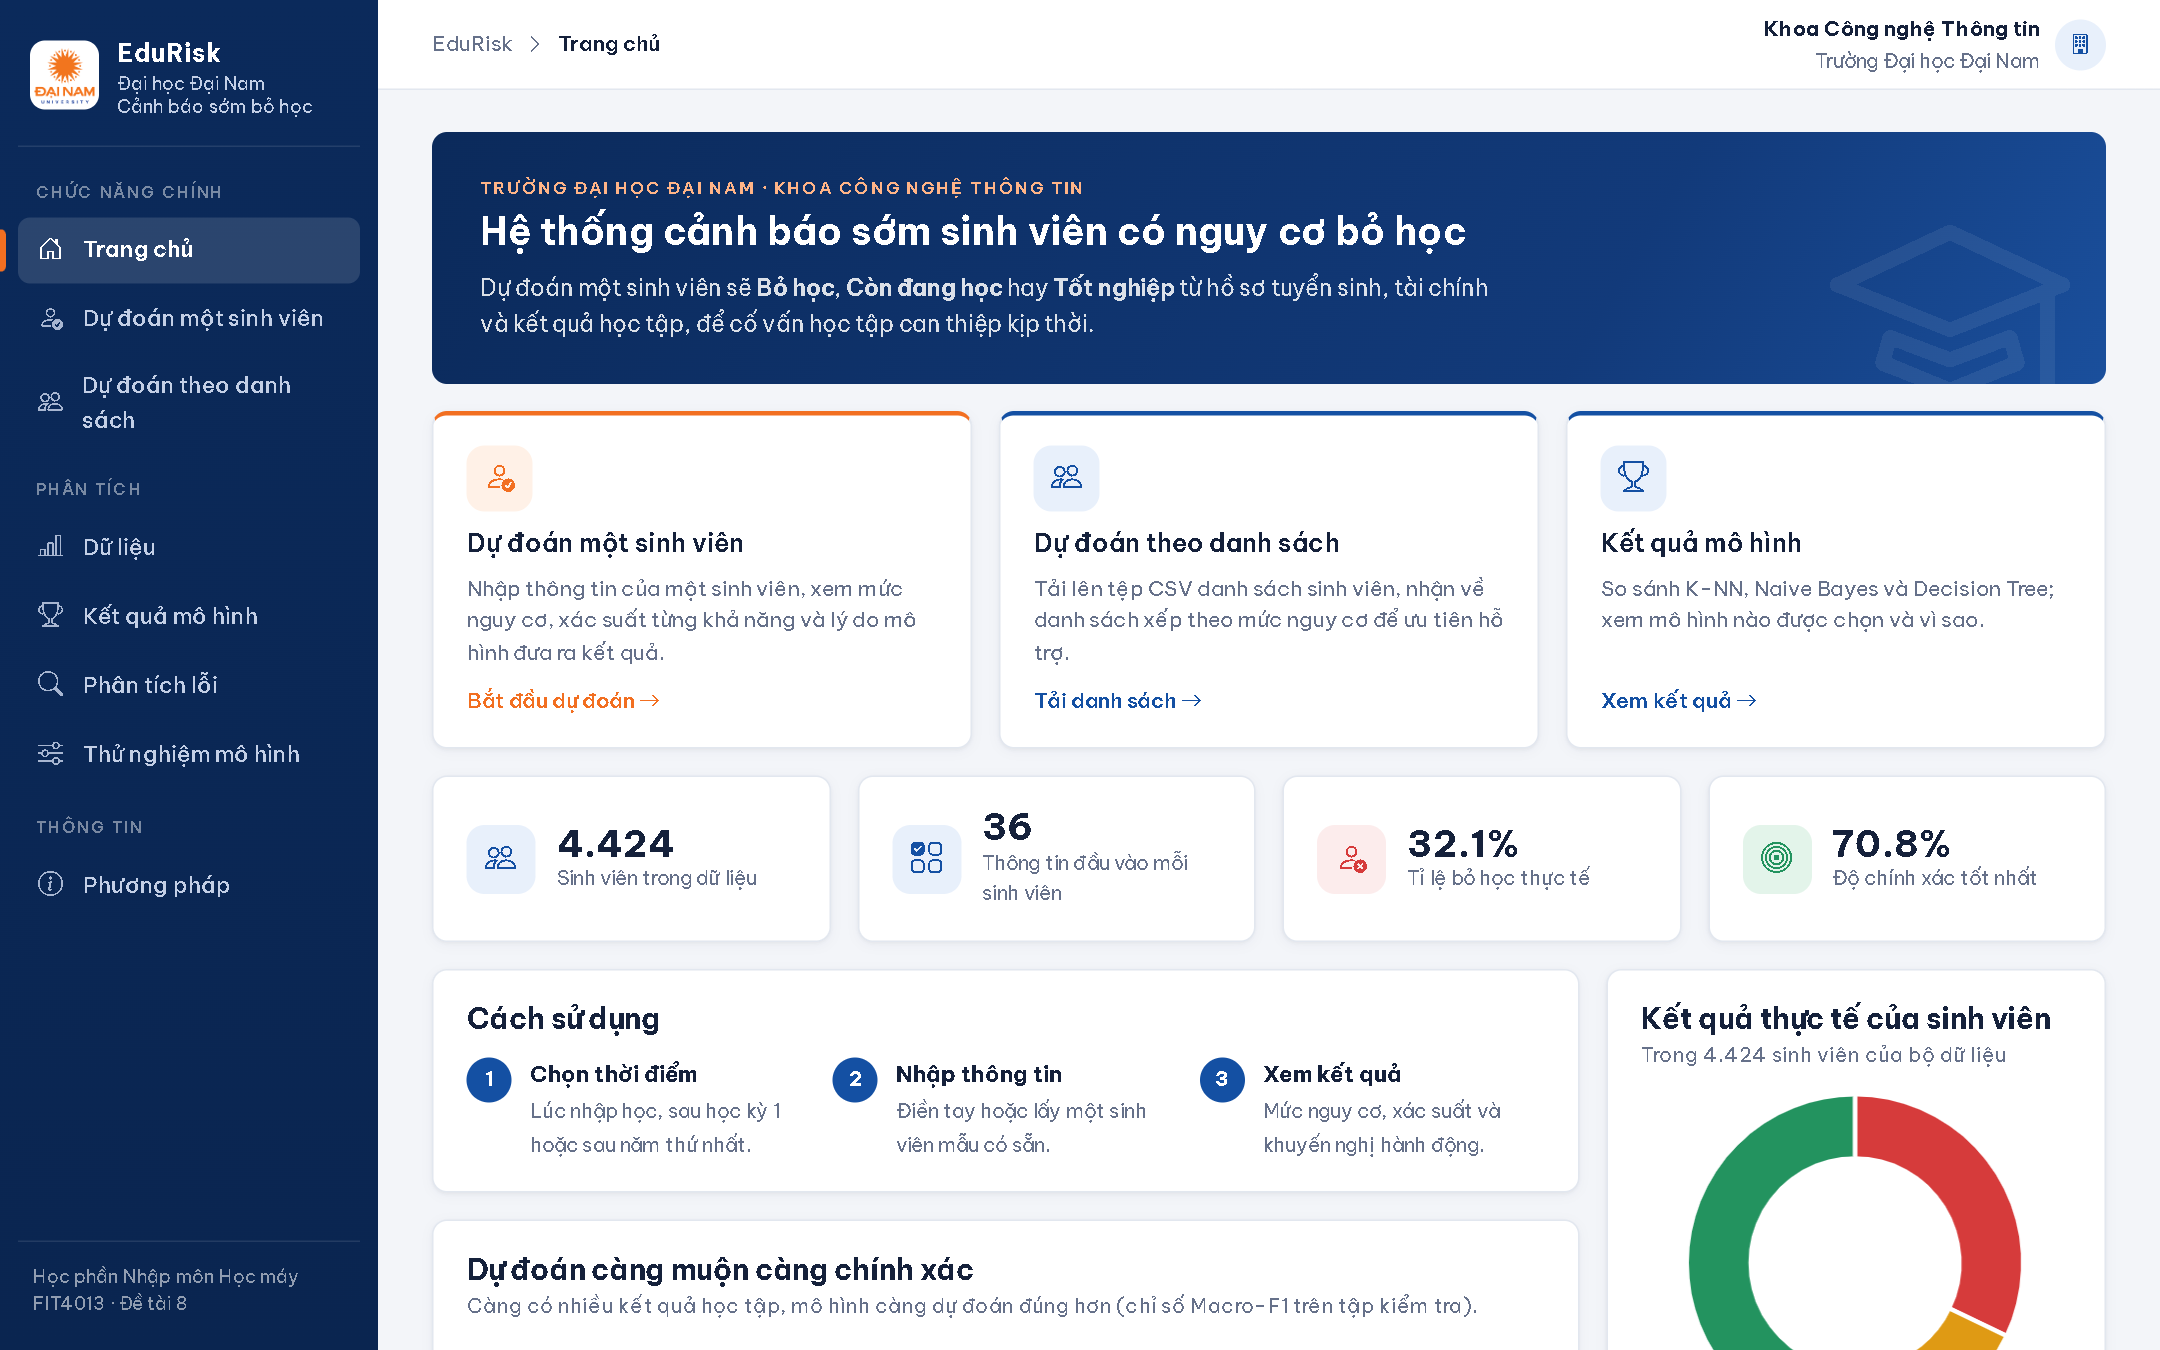
\includegraphics[width=0.97\textwidth]{ui_home.png}}
\caption{Trang chủ của ứng dụng EduRisk}\label{fig:ui-home}
\end{figure}

\begin{table}[H]
\centering\footnotesize
\caption{Các chức năng của ứng dụng web}\label{tab:pages}
\begin{tabularx}{\textwidth}{@{}p{4.2cm}X@{}}
\toprule
\textbf{Trang} & \textbf{Chức năng}\\
\midrule
Dự đoán một sinh viên & Chọn thời điểm, nhập thông tin (hoặc lấy sinh viên mẫu từ tập kiểm tra), nhận mức nguy cơ, xác suất ba lớp, khuyến nghị và giải thích\\
Dự đoán theo danh sách & Tải lên tệp CSV, kiểm tra từng dòng, trả về danh sách xếp theo xác suất bỏ học, lọc theo mức nguy cơ, tải kết quả\\
Dữ liệu & Phân phối từng đặc trưng theo lớp, tương quan, chất lượng dữ liệu, thống kê mô tả\\
Kết quả mô hình & Bảng 39 cấu hình, so sánh luồng, mặc định/tinh chỉnh, khảo sát siêu tham số\\
Phân tích lỗi & Độ quan trọng đặc trưng, cặp nhầm lẫn, tỉ lệ lỗi theo nhóm, các ca sai tự tin\\
Thử nghiệm mô hình & Tự chọn thuật toán, luồng, tham số để huấn luyện ngay; kiểm thử ba mô hình đã lưu\\
\bottomrule
\end{tabularx}
\end{table}

\textbf{Mức nguy cơ} được suy ra từ xác suất bỏ học $p$: \emph{Nguy cơ cao} nếu $p \ge 0{,}5$, \emph{Cần theo dõi} nếu
$0{,}3 \le p < 0{,}5$, còn lại là \emph{Nguy cơ thấp}. Ngưỡng 0,3 thấp hơn 0,5 để không bỏ sót những sinh viên chưa chắc chắn
nhưng đáng được quan tâm.

\textbf{Giải thích dự đoán} theo ba cách bổ sung cho nhau:
(i) so sánh các chỉ số chính của sinh viên với trung bình từng lớp;
(ii) \emph{đường đi quyết định} trên cây: các ngưỡng đã chuẩn hóa được đổi về đơn vị gốc ($\text{ngưỡng}\times\sigma + \mu$)
để người dùng đọc được, ví dụ ``số môn đạt HK2 $\le$ 3,5'';
(iii) 7 sinh viên giống nhất trong tập huấn luyện cùng kết cục thực tế của họ.

Hình~\ref{fig:ui-predict} minh họa chức năng dự đoán một sinh viên ở kịch bản sau học kỳ 1. Người dùng chọn ``Lấy sinh viên mẫu''
thuộc nhóm Bỏ học; hệ thống điền hồ sơ thật của sinh viên \#4312 trong tập kiểm tra. Mô hình cho xác suất bỏ học 82\%, xếp vào
mức \emph{Nguy cơ cao} và khớp với nhãn thực tế. Hình~\ref{fig:ui-explain} là tab \emph{Luật quyết định} của cùng sinh viên:
cây đi qua 4 điều kiện, trong đó có ``đóng học phí đúng hạn: Không'', và dừng ở một nút lá gồm 35 sinh viên huấn luyện; tính theo trọng số lớp, 82\% trong nút lá này là Bỏ học.

\begin{figure}[H]
\centering\fbox{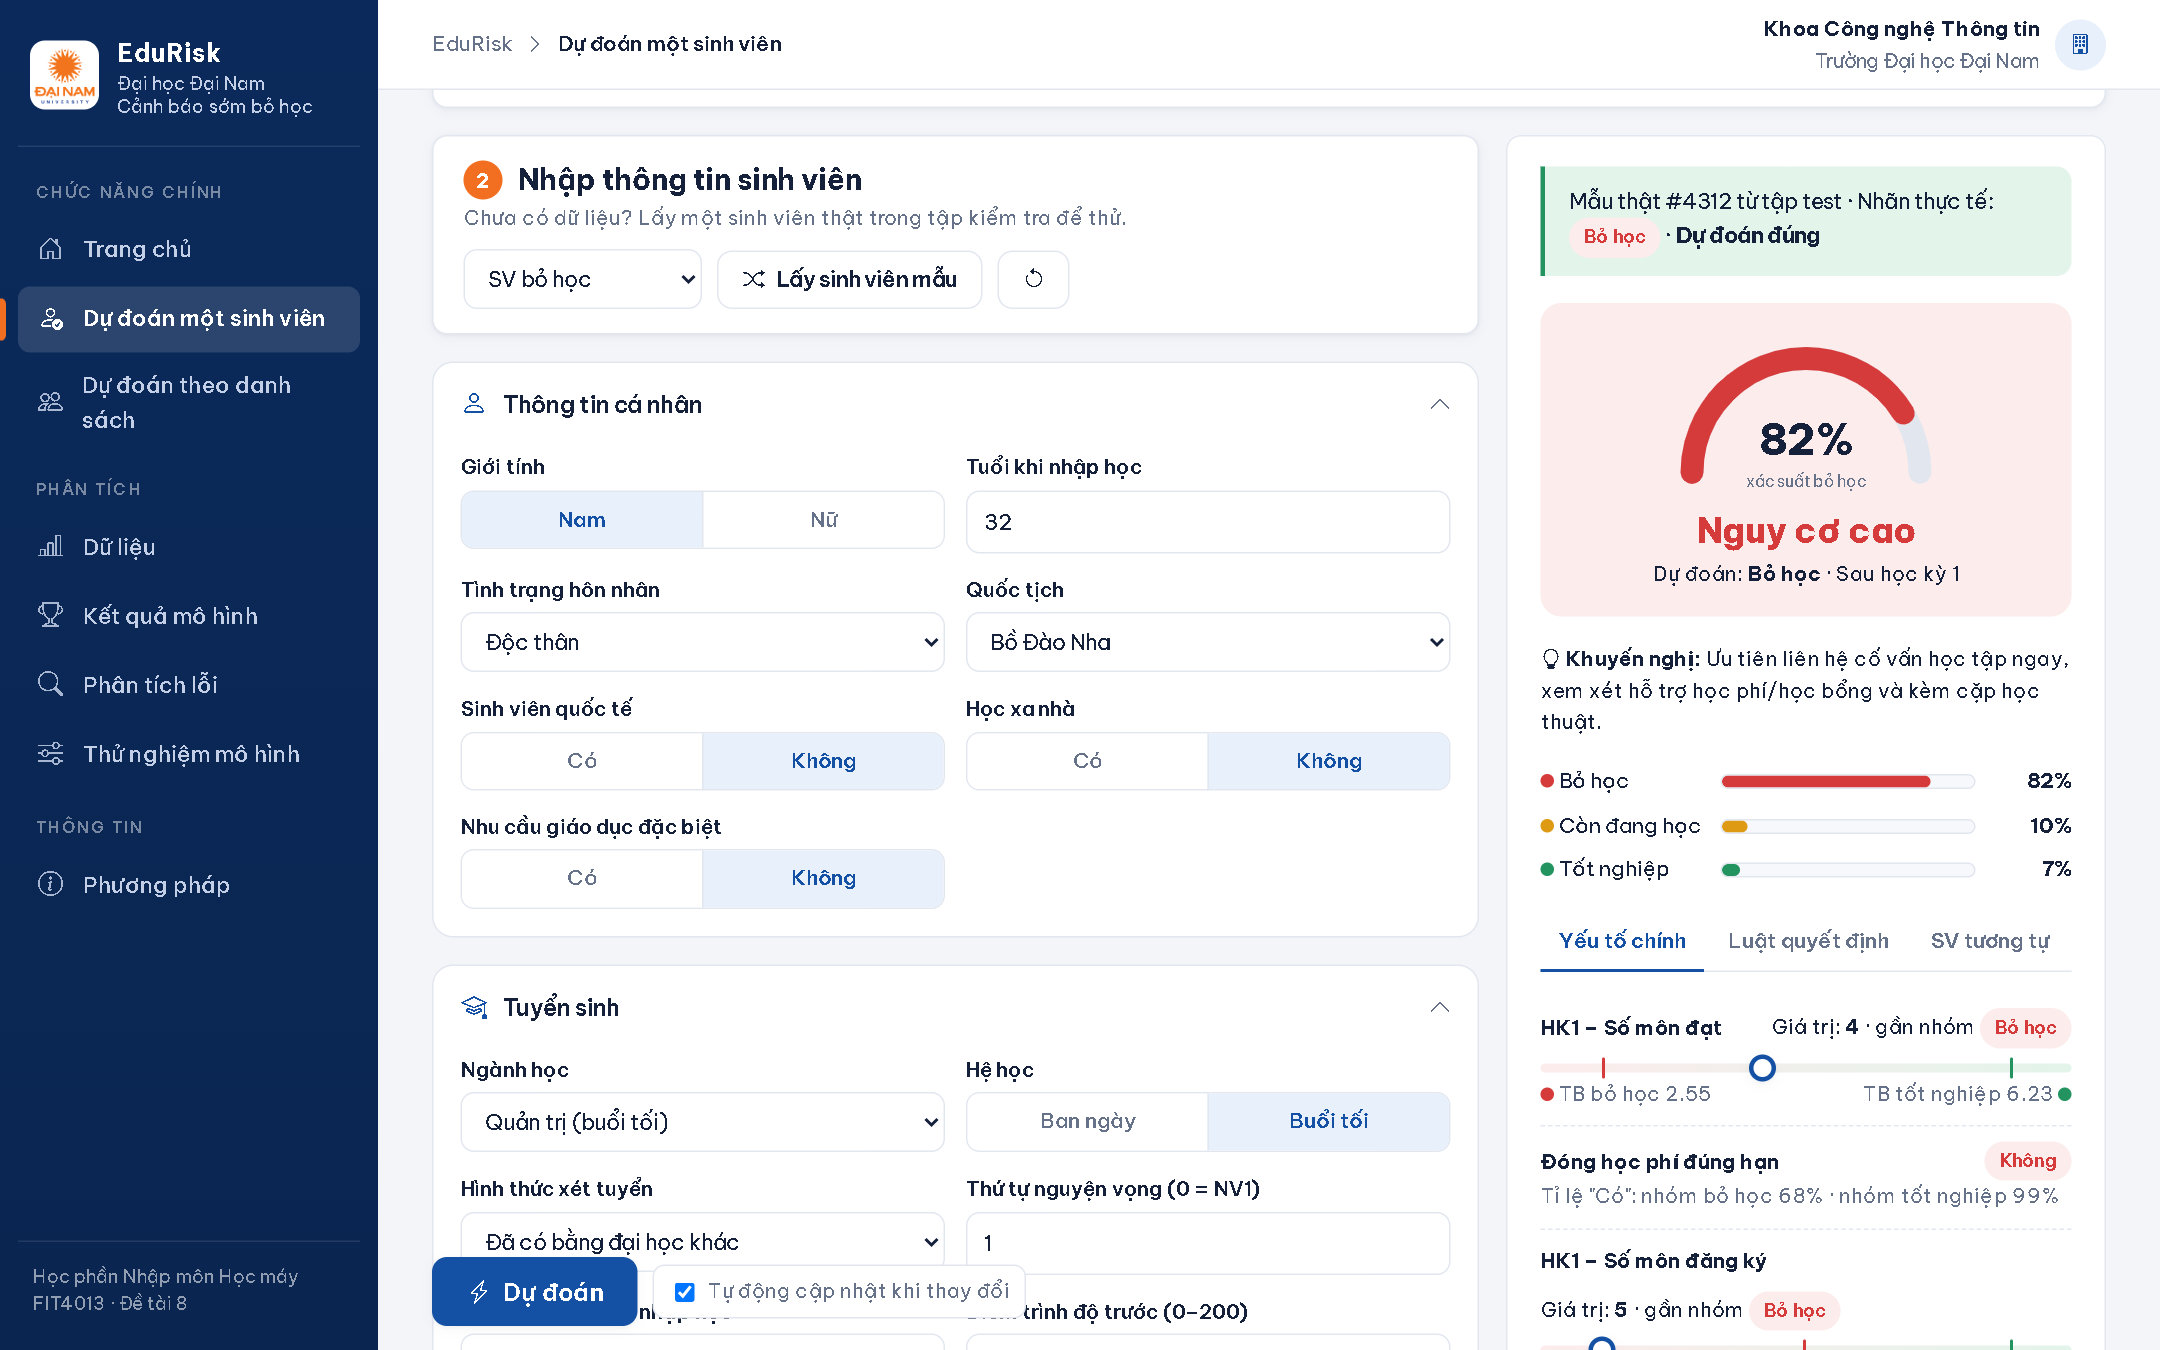
\includegraphics[width=0.97\textwidth]{ui_predict.png}}
\caption{Dự đoán một sinh viên: biểu mẫu nhập thông tin (trái) và kết quả dự đoán (phải)}\label{fig:ui-predict}
\end{figure}

\begin{figure}[H]
\centering\fbox{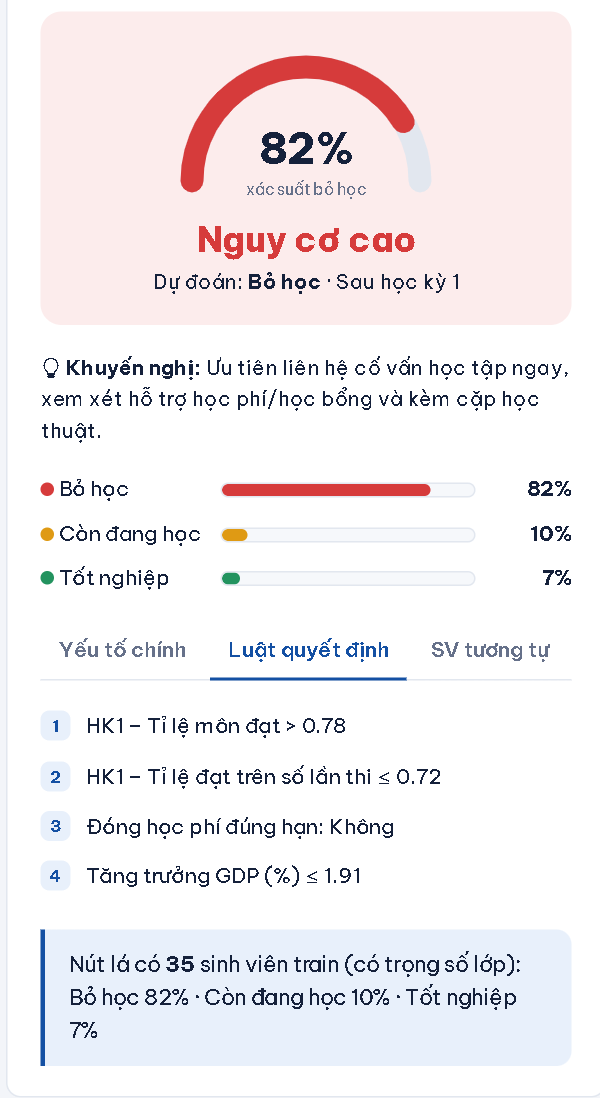
\includegraphics[height=10cm]{ui_explain.png}}
\caption{Giải thích dự đoán bằng đường đi trên cây quyết định}\label{fig:ui-explain}
\end{figure}

\textbf{Kiểm tra đầu vào:} ứng dụng kiểm tra tệp có đủ cột của kịch bản, giá trị phải là số, biến số nằm trong khoảng hợp lý
so với dữ liệu huấn luyện, điểm trung bình học kỳ trong khoảng 0--20 và số môn đạt không vượt quá số môn đăng ký cộng số môn
được công nhận. Mã danh nghĩa chưa từng gặp được One-Hot bỏ qua thay vì gây lỗi. Với dự đoán theo danh sách, dòng lỗi được
báo riêng thay vì làm hỏng cả tệp.

Hình~\ref{fig:ui-batch} là kết quả dự đoán theo danh sách với tệp mẫu 30 sinh viên (10 sinh viên mỗi lớp) lấy từ tập kiểm tra,
ở kịch bản sau năm thứ nhất. Hệ thống xếp danh sách theo xác suất bỏ học giảm dần: 10 sinh viên có nguy cơ cao, 1 cần theo dõi.
Vì tệp có cột \code{Target}, hệ thống đối chiếu với nhãn thật và đánh dấu đúng/sai từng dòng (độ chính xác 66,7\% trên 30 sinh viên này).
Cán bộ có thể lọc theo mức nguy cơ và tải danh sách về dạng CSV.

\begin{figure}[H]
\centering\fbox{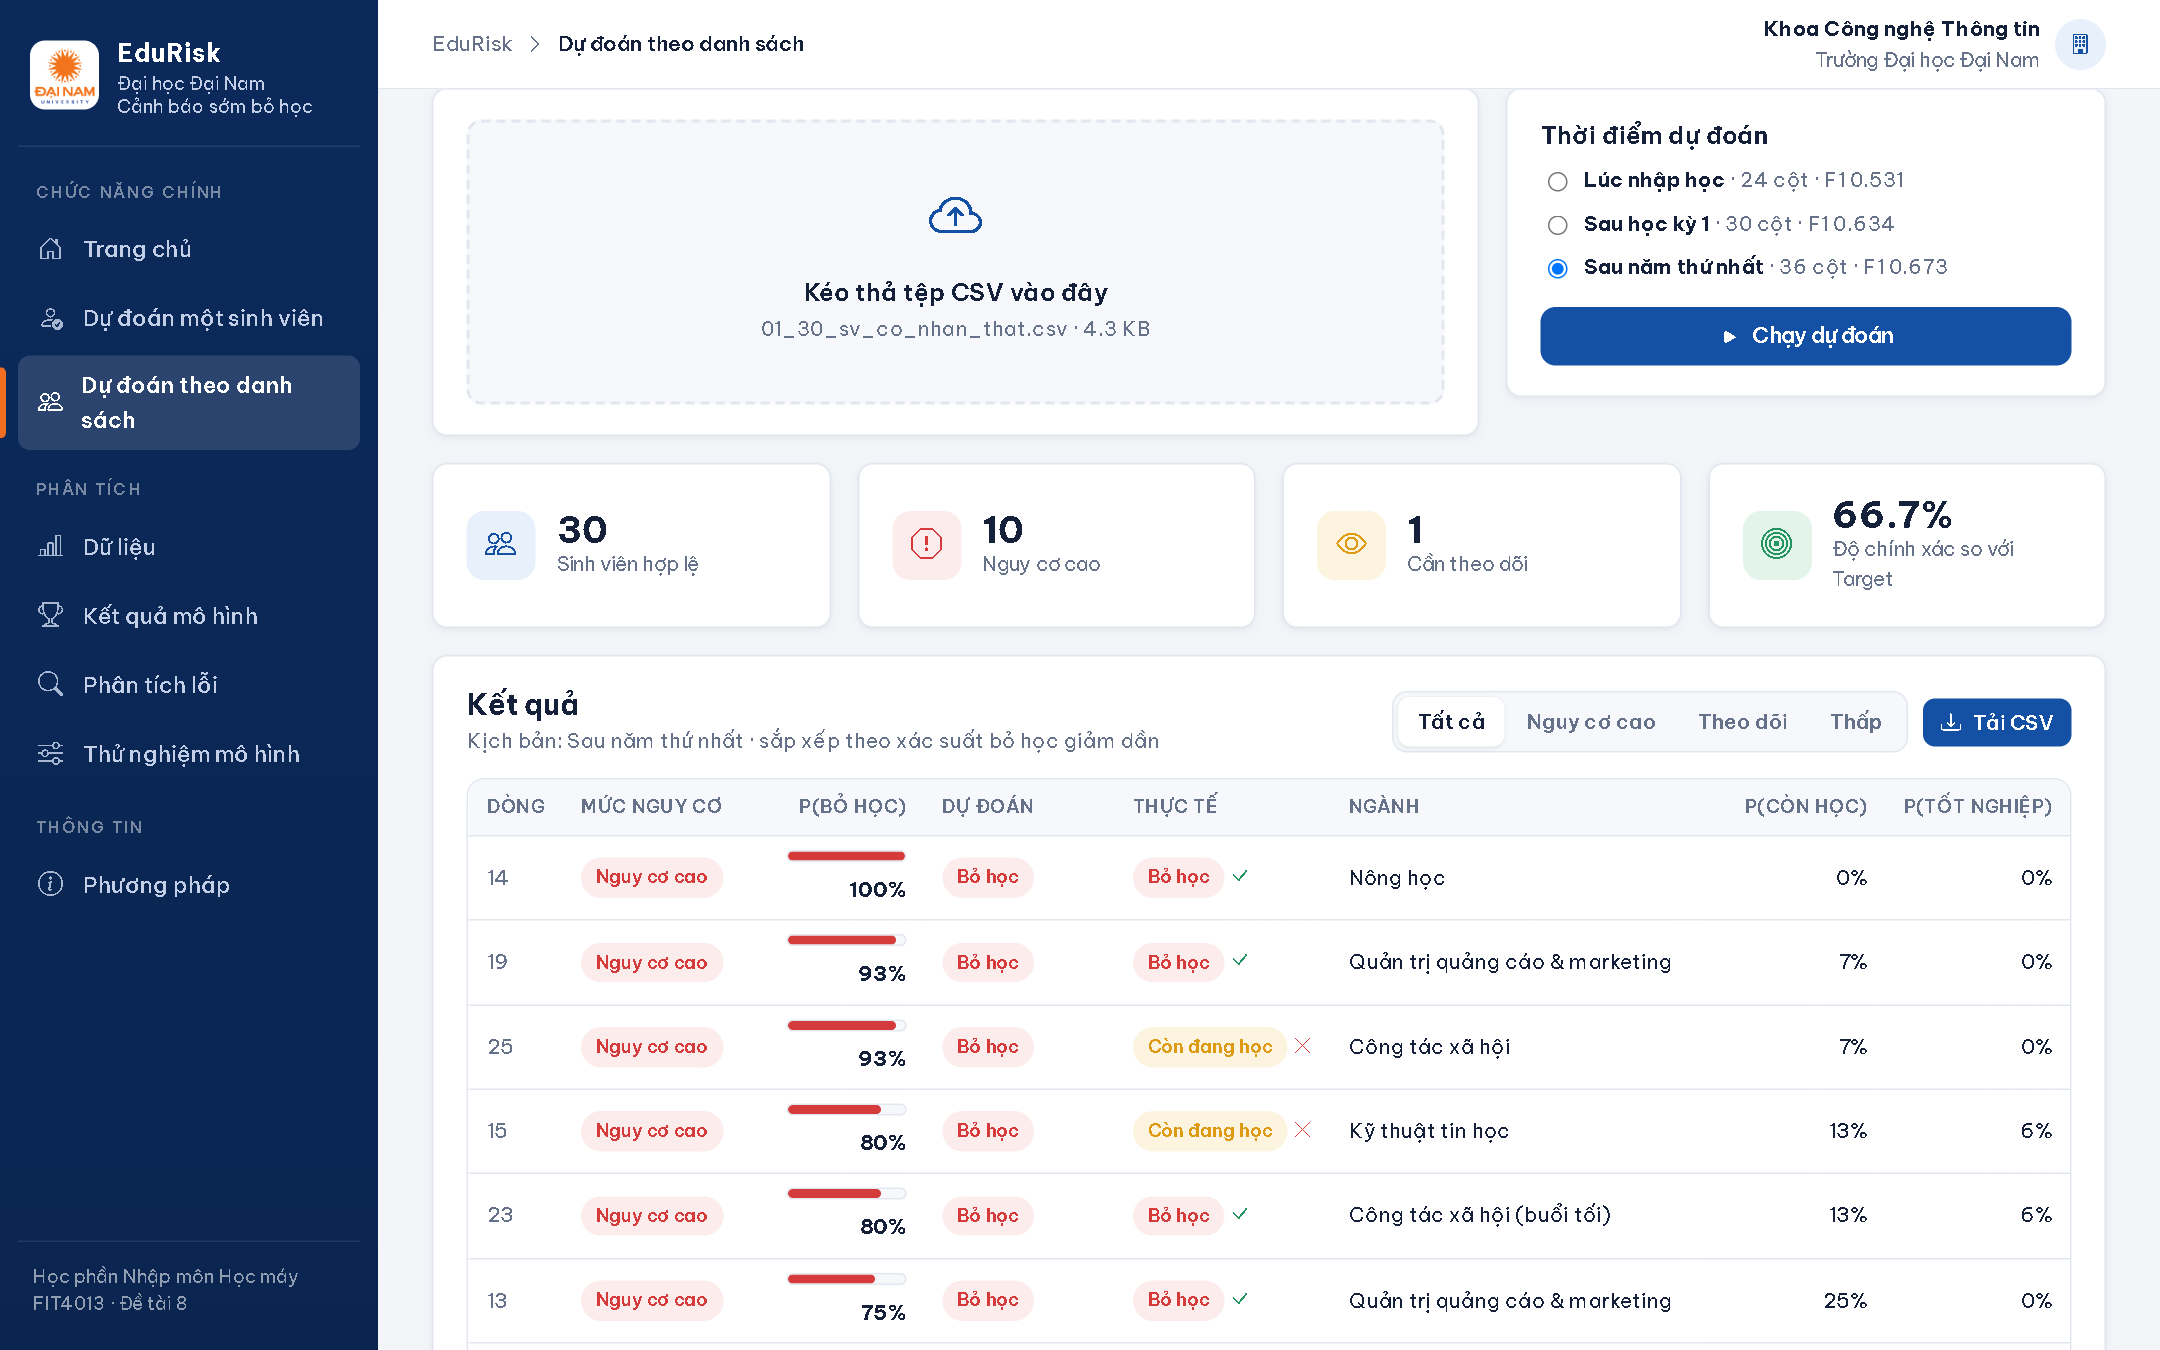
\includegraphics[width=0.97\textwidth]{ui_batch.png}}
\caption{Dự đoán theo danh sách với tệp mẫu 30 sinh viên có nhãn thật}\label{fig:ui-batch}
\end{figure}

Các trang phân tích trình bày lại kết quả thí nghiệm của Chương 4 dưới dạng tương tác. Hình~\ref{fig:ui-exp} là trang Kết quả mô hình,
gồm kết luận chính, thiết lập thí nghiệm và biểu đồ so sánh hai luồng, có thể chuyển giữa ba kịch bản.

\begin{figure}[H]
\centering\fbox{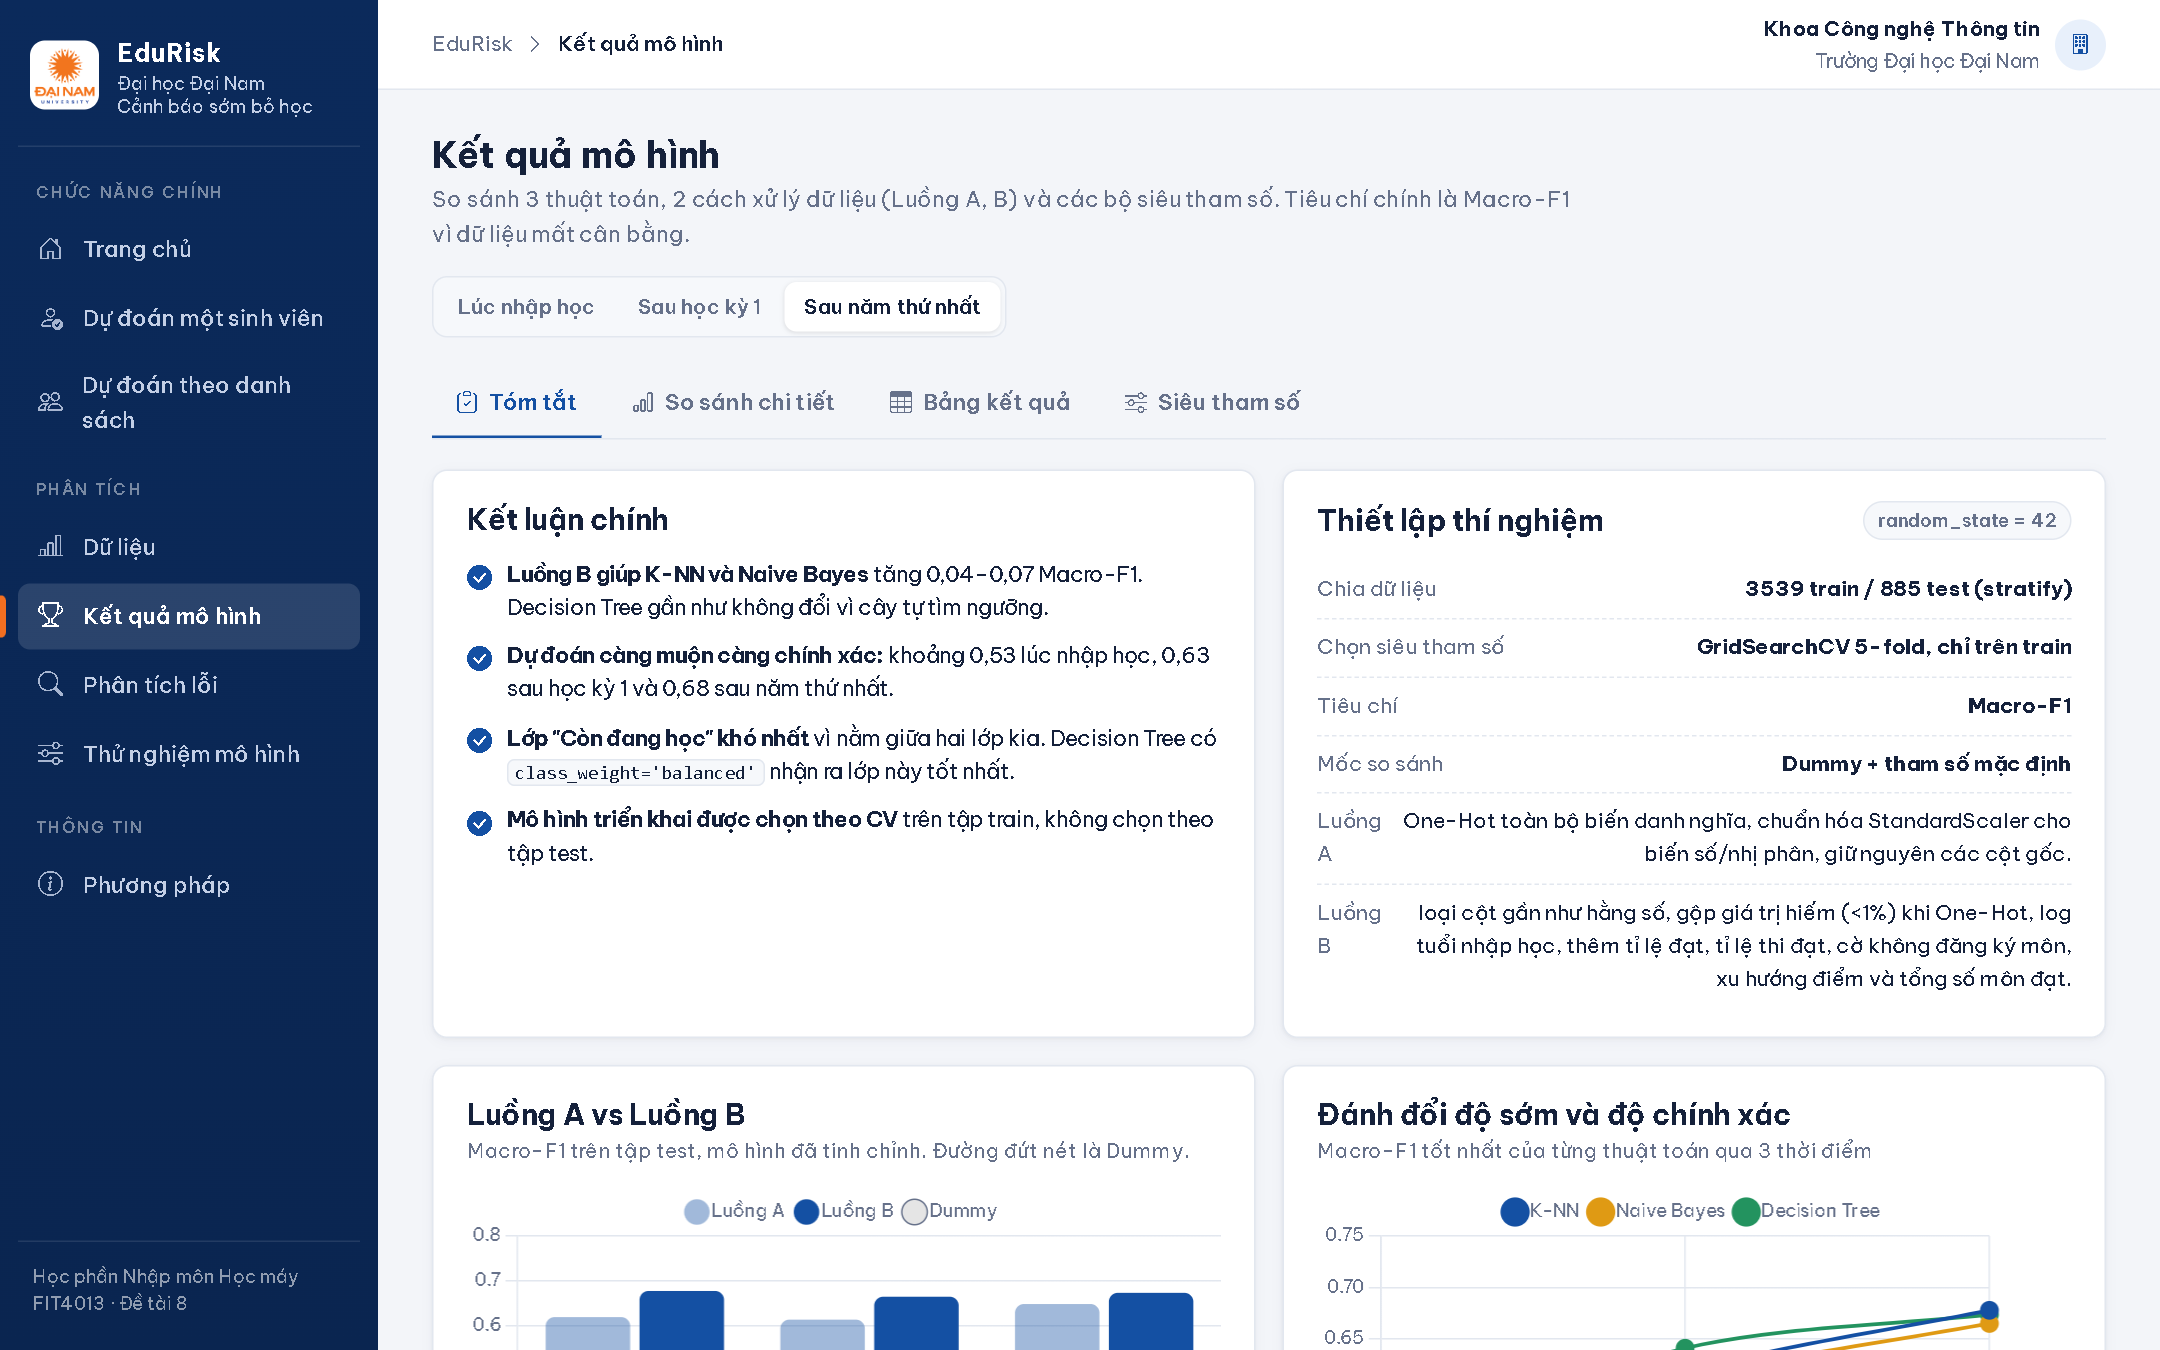
\includegraphics[width=0.97\textwidth]{ui_experiments.png}}
\caption{Trang Kết quả mô hình}\label{fig:ui-exp}
\end{figure}

\section{Khả năng tái lập}
\begin{itemize}
  \item \code{random\_state=42} cố định cho việc chia dữ liệu, kiểm định chéo và mô hình.
  \item \code{python -m src.train} chạy lại toàn bộ thí nghiệm trong khoảng 3 phút (166,6 giây trên máy của nhóm).
  \item \code{python -m src.test\_models} nạp lại ba mô hình, chấm lại trên tập kiểm tra và so khớp với kết quả lúc huấn luyện.
  \item Tệp \code{Run.bat} trên Windows gom các bước cài đặt, huấn luyện, chạy web, kiểm thử vào một menu.
\end{itemize}

% =====================================================================
\chapter{Thử nghiệm và kết quả}
% =====================================================================
\section{Thiết lập thí nghiệm}
\begin{itemize}
  \item \textbf{Dữ liệu:} 3.539 mẫu huấn luyện, 885 mẫu kiểm tra (Bỏ học 284, Còn đang học 159, Tốt nghiệp 442).
  \item \textbf{Không gian thí nghiệm:} 3 kịch bản $\times$ 2 luồng $\times$ 3 thuật toán $\times$ \{mặc định, tinh chỉnh\} = 36 cấu hình,
        cộng 3 baseline Dummy = \textbf{39 cấu hình}.
  \item \textbf{Chỉ số:} \fone{} (chính), accuracy, ROC-AUC một-với-phần-còn-lại, recall và F1 từng lớp.
  \item \textbf{Môi trường:} Python 3.14, scikit-learn 1.9, pandas 3.0, Windows 11.
\end{itemize}

\section{Phương án baseline}
Hai mức baseline được dùng làm mốc:
\begin{enumerate}
  \item \code{DummyClassifier(strategy="most\_frequent")}: luôn đoán Tốt nghiệp. Accuracy 49,9\% nhưng \fone{} chỉ \textbf{0,222}
        vì F1 của hai lớp còn lại bằng 0. Mọi mô hình hữu ích phải vượt xa mốc này.
  \item Mỗi thuật toán với tham số mặc định của scikit-learn: cho biết phần cải thiện đến từ tinh chỉnh.
\end{enumerate}

\section{Kết quả tổng hợp}
\begin{table}[H]
\centering\footnotesize
\caption{Kết quả các mô hình đã tinh chỉnh (CV: trung bình $\pm$ độ lệch chuẩn trên 5 phần; Test: tập kiểm tra). Dòng tô màu là mô hình triển khai.}\label{tab:results}
\setlength{\tabcolsep}{2.5pt}
\begin{tabular}{@{}llllccc@{}}
\toprule
\textbf{Kịch bản} & \textbf{Luồng} & \textbf{Thuật toán} & \textbf{Tham số tốt nhất} & \textbf{CV \fone} & \textbf{Test \fone} & \textbf{Acc.}\\
\midrule
Nhập học & -- & Dummy & most\_frequent & -- & 0,222 & 0,499\\
 & A & K-NN & $k$=5, $p$=2, uniform & 0,513 $\pm$ 0,005 & 0,505 & 0,575\\
 & A & NB & vs=0,01 & 0,527 $\pm$ 0,019 & 0,511 & 0,563\\
\rowcolor{best} & A & DT & d=10, leaf=80, gini, bal. & 0,531 $\pm$ 0,017 & 0,531 & 0,558\\
 & B & K-NN & $k$=5, $p$=2, uniform & 0,528 $\pm$ 0,009 & 0,510 & 0,572\\
 & B & NB & vs=0,01 & 0,531 $\pm$ 0,015 & 0,521 & 0,557\\
 & B & DT & d=10, leaf=80, gini, bal. & 0,531 $\pm$ 0,017 & 0,531 & 0,558\\
\midrule
Sau HK1 & -- & Dummy & most\_frequent & -- & 0,222 & 0,499\\
 & A & K-NN & $k$=7, $p$=1, uniform & 0,584 $\pm$ 0,016 & 0,580 & 0,678\\
 & A & NB & vs=0,1 & 0,567 $\pm$ 0,024 & 0,545 & 0,643\\
 & A & DT & d=8, leaf=20, entropy, bal. & 0,644 $\pm$ 0,016 & 0,641 & 0,676\\
 & B & K-NN & $k$=7, $p$=1, distance & 0,627 $\pm$ 0,011 & 0,618 & 0,707\\
 & B & NB & vs=0,1 & 0,630 $\pm$ 0,020 & 0,611 & 0,690\\
\rowcolor{best} & B & DT & d=4, leaf=10, entropy, bal. & 0,652 $\pm$ 0,010 & 0,634 & 0,670\\
\midrule
Sau năm 1 & -- & Dummy & most\_frequent & -- & 0,222 & 0,499\\
 & A & K-NN & $k$=11, $p$=1, uniform & 0,620 $\pm$ 0,021 & 0,619 & 0,718\\
 & A & NB & vs=0,1 & 0,622 $\pm$ 0,020 & 0,614 & 0,689\\
 & A & DT & d=6, leaf=40, entropy, bal. & 0,676 $\pm$ 0,019 & 0,649 & 0,671\\
 & B & K-NN & $k$=7, $p$=1, distance & 0,679 $\pm$ 0,018 & \textbf{0,678} & \textbf{0,756}\\
 & B & NB & vs=0,1 & 0,675 $\pm$ 0,010 & 0,665 & 0,724\\
\rowcolor{best} & B & DT & d=6, leaf=20, gini, bal. & \textbf{0,685 $\pm$ 0,010} & 0,673 & 0,708\\
\bottomrule
\end{tabular}
\\[2pt]{\footnotesize vs = var\_smoothing; d = max\_depth; leaf = min\_samples\_leaf; bal. = class\_weight balanced.}
\end{table}

Mọi mô hình đều vượt xa baseline Dummy (0,222). \fone{} của mô hình triển khai tăng dần theo lượng thông tin:
0,531 $\rightarrow$ 0,634 $\rightarrow$ 0,673. Ở kịch bản lúc nhập học, Decision Tree của hai luồng cho kết quả giống hệt
nhau; khi bằng điểm, chương trình giữ cấu hình xuất hiện trước (Luồng A).

\section{Ảnh hưởng của tinh chỉnh siêu tham số}
\begin{table}[H]
\centering\small
\caption{\fone{} trên tập kiểm tra: tham số mặc định $\rightarrow$ đã tinh chỉnh}\label{tab:tuning}
\setlength{\tabcolsep}{4.5pt}
\begin{tabular}{@{}lcccccc@{}}
\toprule
 & \multicolumn{2}{c}{\textbf{K-NN}} & \multicolumn{2}{c}{\textbf{Naive Bayes}} & \multicolumn{2}{c}{\textbf{Decision Tree}}\\
\cmidrule(lr){2-3}\cmidrule(lr){4-5}\cmidrule(lr){6-7}
\textbf{Kịch bản / Luồng} & Mặc định & Tinh chỉnh & Mặc định & Tinh chỉnh & Mặc định & Tinh chỉnh\\
\midrule
Nhập học / A & 0,505 & 0,505 & 0,217 & 0,511 & 0,503 & 0,531\\
Nhập học / B & 0,510 & 0,510 & 0,242 & 0,521 & 0,483 & 0,531\\
Sau HK1 / A  & 0,602 & 0,580 & 0,217 & 0,545 & 0,591 & 0,641\\
Sau HK1 / B  & 0,636 & 0,618 & 0,262 & 0,611 & 0,589 & 0,634\\
Sau năm 1 / A & 0,618 & 0,619 & 0,217 & 0,614 & 0,608 & 0,649\\
Sau năm 1 / B & 0,661 & 0,678 & 0,320 & 0,665 & 0,626 & 0,673\\
\bottomrule
\end{tabular}
\end{table}
\begin{figure}[H]
\centering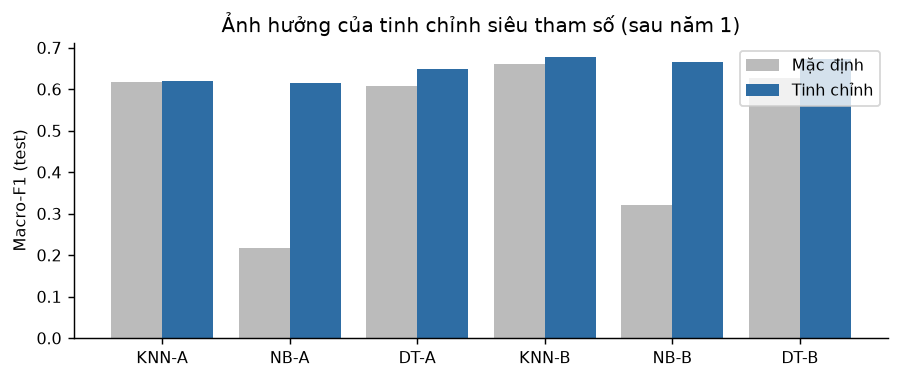
\includegraphics[width=0.8\textwidth]{result_default_vs_tuned.png}
\caption{So sánh tham số mặc định và tinh chỉnh (kịch bản sau năm 1)}\label{fig:tuning}
\end{figure}
\begin{itemize}
  \item \textbf{Naive Bayes} được lợi nhiều nhất: từ khoảng 0,22 (ngang baseline) lên 0,51--0,67 khi \code{var\_smoothing} tăng từ $10^{-9}$ lên 0,01--0,1.
  \item \textbf{Decision Tree} tăng 0,03--0,05 nhờ giới hạn độ sâu, số mẫu ở lá và gán trọng số cân bằng cho các lớp. Cây mặc định mọc hết cỡ nên học thuộc dữ liệu huấn luyện.
  \item \textbf{K-NN} gần như không đổi; ở kịch bản sau HK1, điểm test sau tinh chỉnh còn thấp hơn mặc định khoảng 0,02 dù CV cao hơn. Mức chênh này nằm trong độ dao động của CV ($\pm$0,01--0,02), cho thấy không nên đọc quá kỹ các khác biệt nhỏ trên một tập kiểm tra 885 mẫu.
\end{itemize}

\begin{figure}[H]
\centering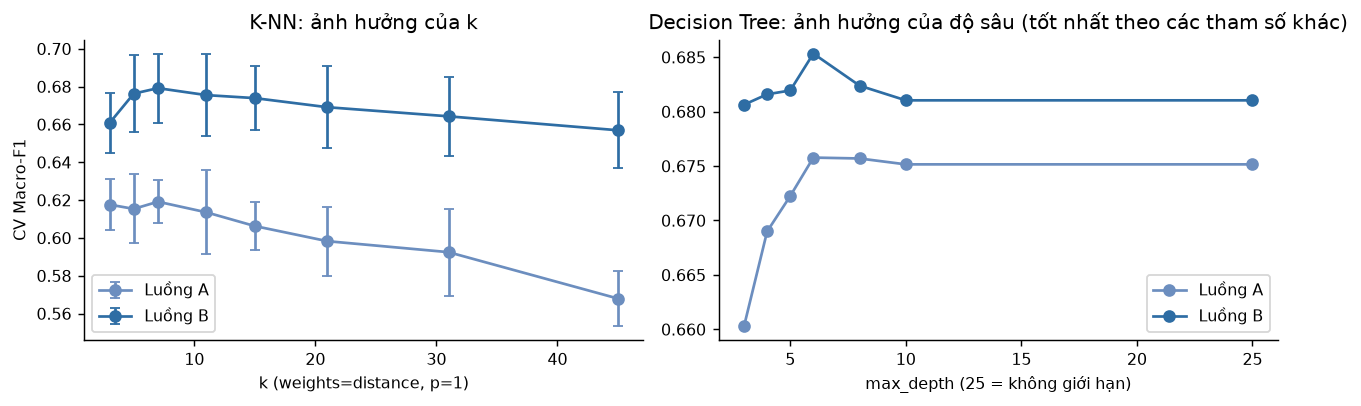
\includegraphics[width=\textwidth]{result_hyperparameters.png}
\caption{Ảnh hưởng của $k$ (K-NN) và độ sâu cây (Decision Tree) đến CV \fone{}}\label{fig:hparams}
\end{figure}
Với K-NN (kịch bản sau năm 1, Luồng B), CV \fone{} tăng từ 0,661 ở $k=3$ lên cao nhất 0,679 ở $k=7$, rồi giảm dần còn 0,657
ở $k=45$: $k$ quá nhỏ thì nhạy với nhiễu, $k$ quá lớn thì lớp thiểu số Còn đang học bị các lớp đông hơn lấn át.
Với Decision Tree, khi các tham số khác đã chọn tốt nhất, độ sâu chỉ làm CV dao động trong khoảng 0,681--0,685 (sau HK1: 0,636--0,652),
vì \code{min\_samples\_leaf} đã đóng vai trò chống quá khớp. Ngược lại, cây mặc định (không giới hạn độ sâu, lá tối thiểu 1 mẫu)
thấp hơn cây tinh chỉnh 0,03--0,05 (Bảng~\ref{tab:tuning}), cho thấy quá khớp xảy ra khi bỏ cả hai ràng buộc.

\section{So sánh hai luồng tiền xử lý}
\begin{figure}[H]
\centering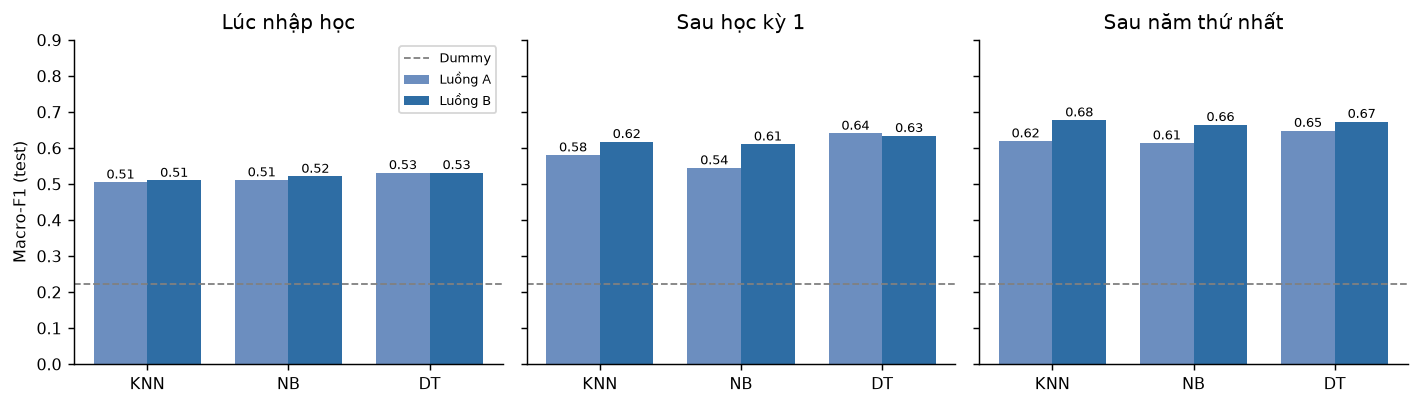
\includegraphics[width=\textwidth]{result_flow_comparison.png}
\caption{\fone{} trên tập kiểm tra của Luồng A và Luồng B theo từng kịch bản}\label{fig:flow}
\end{figure}
Ở kịch bản sau HK1 và sau năm 1, Luồng B tăng \fone{} của K-NN thêm 0,038 và 0,059, của Naive Bayes thêm 0,066 và 0,051.
Lúc nhập học mức tăng chỉ khoảng 0,005--0,01, vì các đặc trưng mới đều dựa trên kết quả học kỳ. Decision Tree hầu như không
thay đổi (chênh lệch dưới 0,03 theo cả hai chiều).

\section{Mô hình triển khai}
\begin{table}[H]
\centering\small
\caption{Chỉ số chi tiết của ba mô hình triển khai trên tập kiểm tra}\label{tab:deployed}
\setlength{\tabcolsep}{4pt}
\begin{tabular}{@{}lccccccc@{}}
\toprule
\textbf{Kịch bản} & \textbf{Acc.} & \textbf{\fone} & \textbf{AUC} & \multicolumn{3}{c}{\textbf{Recall}} & \textbf{F1 Còn học}\\
\cmidrule(lr){5-7}
 & & & & Bỏ học & Còn học & Tốt nghiệp & \\
\midrule
Nhập học (DT-A)  & 0,558 & 0,531 & 0,727 & 0,592 & 0,472 & 0,568 & 0,357\\
Sau HK1 (DT-B)   & 0,670 & 0,634 & 0,830 & 0,669 & 0,553 & 0,713 & 0,413\\
Sau năm 1 (DT-B) & 0,708 & 0,673 & 0,855 & 0,627 & 0,660 & 0,778 & 0,492\\
\bottomrule
\end{tabular}
\end{table}

\begin{figure}[H]
\centering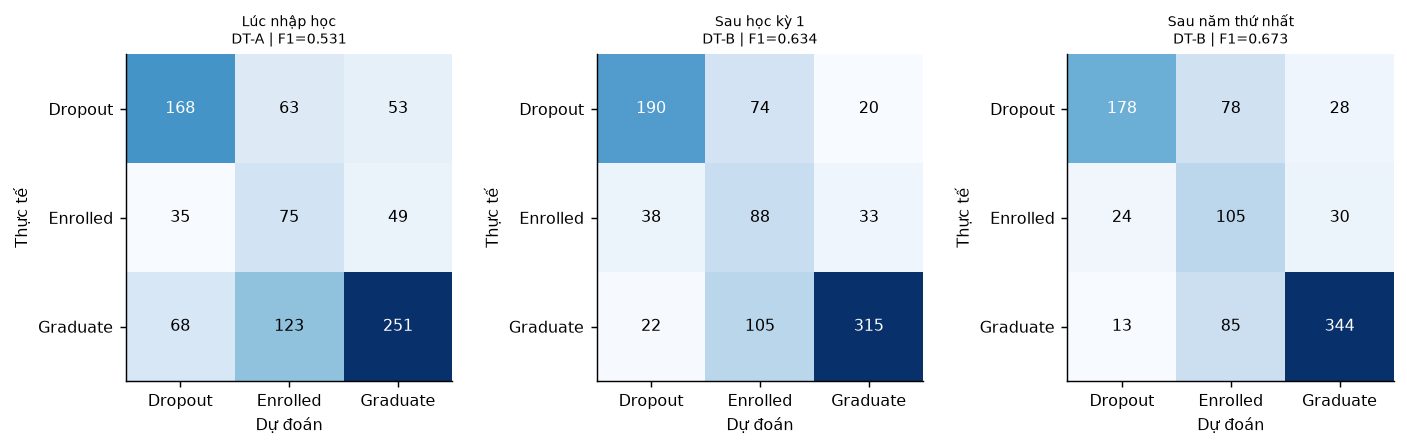
\includegraphics[width=\textwidth]{result_confusion_matrices.png}
\caption{Ma trận nhầm lẫn của ba mô hình triển khai trên tập kiểm tra}\label{fig:cm}
\end{figure}

\begin{table}[H]
\centering\small
\caption{Ma trận nhầm lẫn của mô hình sau năm 1 (hàng: thực tế, cột: dự đoán)}\label{tab:cmfull}
\begin{tabular}{@{}lccc|c@{}}
\toprule
 & Bỏ học & Còn học & Tốt nghiệp & Tổng\\
\midrule
Bỏ học     & \textbf{178} & 78 & 28 & 284\\
Còn học    & 24 & \textbf{105} & 30 & 159\\
Tốt nghiệp & 13 & 85 & \textbf{344} & 442\\
\bottomrule
\end{tabular}
\end{table}
Nhờ \code{class\_weight="balanced"}, cây có recall cân đối giữa ba lớp; lớp Còn đang học đạt recall 0,66 so với 0,26--0,36
của K-NN. Đổi lại, cây dự đoán Còn đang học khá nhiều nên precision của lớp này thấp. Nhầm lẫn nghiêm trọng nhất về mặt
thực tế, tức sinh viên Bỏ học bị đoán là Tốt nghiệp, chỉ có 28/284 trường hợp (9,9\%).

\section{Mức độ quan trọng của đặc trưng}
\begin{figure}[H]
\centering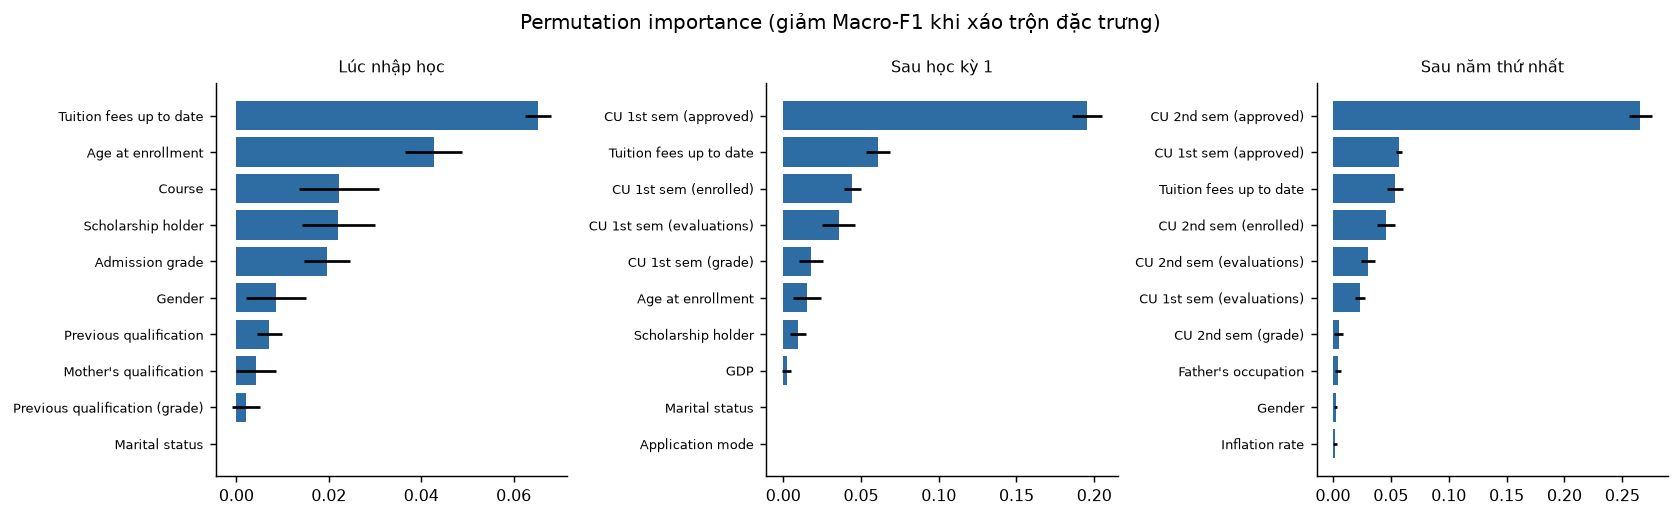
\includegraphics[width=\textwidth]{result_permutation_importance.png}
\caption{Permutation importance: mức giảm \fone{} khi xáo trộn từng đặc trưng (8 lần lặp)}\label{fig:imp}
\end{figure}
Permutation importance \cite{breiman2001} được tính trên tập kiểm tra theo \fone{}, áp dụng được cho mọi loại mô hình.
\begin{itemize}
  \item \textbf{Lúc nhập học:} đóng học phí đúng hạn (0,065), tuổi nhập học (0,043), ngành học, học bổng, điểm xét tuyển.
  \item \textbf{Sau HK1:} số học phần đạt HK1 chiếm ưu thế (0,195), tiếp theo là học phí (0,061) và số học phần đăng ký.
  \item \textbf{Sau năm 1:} số học phần đạt HK2 (0,266) vượt xa các đặc trưng khác.
\end{itemize}
Các biến về gia đình (học vấn, nghề nghiệp của cha mẹ) và kinh tế vĩ mô có ảnh hưởng rất nhỏ. Nhóm kiểm tra thêm: thay các
cột này bằng giá trị mặc định làm \fone{} thay đổi không quá 0,006.

% =====================================================================
\chapter{Thảo luận và so sánh}\label{ch:discuss}
% =====================================================================
\section{Ưu, nhược điểm của các phương án}
\begin{table}[H]
\centering\small
\caption{So sánh ba thuật toán trên bài toán này}\label{tab:proscons}
\begin{tabularx}{\textwidth}{@{}lXX@{}}
\toprule
 & \textbf{Ưu điểm} & \textbf{Nhược điểm}\\
\midrule
K-NN & Accuracy cao nhất sau năm 1 (0,756); giải thích bằng ví dụ tương tự & Recall lớp Còn đang học thấp (0,26--0,36); rất phụ thuộc tiền xử lý; dự đoán chậm hơn khi dữ liệu lớn\\
Naive Bayes & Huấn luyện tức thì; cho xác suất; cải thiện rõ nhờ Luồng B & Giả định độc lập bị vi phạm nặng; mặc định gần như vô dụng nếu không chỉnh \code{var\_smoothing}\\
Decision Tree & CV \fone{} cao nhất ở cả ba kịch bản; recall cân bằng; giải thích bằng luật; không cần chuẩn hóa & Không ổn định (dữ liệu thay đổi nhỏ có thể đổi cấu trúc cây); dễ quá khớp nếu không giới hạn\\
\bottomrule
\end{tabularx}
\end{table}
Mục tiêu của hệ thống là \emph{phát hiện} sinh viên có nguy cơ và \emph{giải thích} cho cán bộ, nên Decision Tree là lựa chọn
hợp lý: điểm CV cao nhất, recall các lớp thiểu số tốt hơn và có luật quyết định dễ đọc. Sau năm 1, K-NN Luồng B có điểm
test cao hơn cây 0,005, nhưng mức chênh này nhỏ hơn độ lệch chuẩn của CV và mô hình được chọn trước khi xem tập kiểm tra.

\section{Tại sao Luồng B giúp K-NN và Naive Bayes nhưng không giúp Decision Tree}
\begin{itemize}
  \item \textbf{K-NN} tính khoảng cách trên mọi cột như nhau. Ở kịch bản sau năm 1, Luồng A tạo ra 247 cột sau mã hóa, phần lớn là cột One-Hot của mã hiếm; Luồng B chỉ còn 111 cột.
        Các cột này làm loãng khoảng cách, khiến hai sinh viên có kết quả học tập rất khác nhau vẫn được coi là ``gần''.
        Bỏ cột nhiễu, gộp mã hiếm và thêm tỉ lệ đạt giúp khoảng cách phản ánh đúng hơn mức độ giống nhau về học tập.
  \item \textbf{Naive Bayes} giả định mỗi đặc trưng có phân phối chuẩn. Tuổi lệch phải và ``số 0 trá hình'' phá vỡ giả định đó.
        Phép log và cờ \code{no\_enrolment} làm phân phối gần chuẩn hơn; tỉ lệ đạt gói nhiều cột tương quan thành một tín hiệu.
  \item \textbf{Decision Tree} chọn ngưỡng trên từng cột riêng lẻ, không bị ảnh hưởng bởi thang đo hay cột nhiễu (cây chỉ không chọn cột đó).
        Cây cũng tự tìm được các ngưỡng tương đương tỉ lệ đạt bằng cách kết hợp nhiều lần chia, nên đặc trưng mới không bổ sung nhiều thông tin.
\end{itemize}

\section{Tại sao Naive Bayes mặc định thất bại}
Với cột One-Hot, trong một lớp nhiều cột có giá trị gần như toàn 0, nên phương sai xấp xỉ 0. Giá trị mặc định
\code{var\_smoothing}$=10^{-9}$ quá nhỏ: một giá trị 1 bất kỳ ở cột đó cho mật độ xác suất gần như bằng 0, và một cột duy nhất
có thể áp đảo cả tích xác suất. Kết quả là mô hình dồn dự đoán vào một lớp (\fone{} khoảng 0,22, accuracy 24\%).
Tăng \code{var\_smoothing} lên 0,01--0,1 làm mượt các phân phối này và đưa \fone{} lên 0,51--0,67.

\section{Phân tích dự đoán sai}
\textbf{Các cặp nhầm lẫn.} Với mô hình sau năm 1, 258/885 mẫu bị đoán sai. Hai cặp nhầm lẫn lớn nhất đều liên quan tới
lớp Còn đang học: Tốt nghiệp $\rightarrow$ Còn học (85) và Bỏ học $\rightarrow$ Còn học (78). Lúc nhập học, cặp lớn nhất là
Tốt nghiệp $\rightarrow$ Còn học (123/391 lỗi).

\textbf{Vì sao lớp Còn đang học khó?} Về bản chất, ``Còn đang học'' là trạng thái \emph{chưa kết thúc} tại thời điểm thu thập dữ liệu:
một phần sẽ tốt nghiệp muộn, một phần sẽ bỏ học. Đặc trưng của họ vì vậy nằm giữa hai lớp kia (Mục 1.4.3). Lớp này cũng
ít mẫu nhất (17,9\%).

\textbf{Tỉ lệ lỗi theo nhóm} (mô hình sau năm 1):
\begin{itemize}
  \item Sinh viên \emph{có học bổng}: lỗi 19,0\%, so với 32,2\% ở nhóm không có học bổng. Học bổng gắn với kết quả học tốt nên dễ dự đoán là Tốt nghiệp.
  \item Sinh viên \emph{nợ học phí}: lỗi chỉ 18,3\% (so với 30,7\%), vì phần lớn nhóm này bỏ học và mô hình nhận ra tín hiệu này rất rõ.
  \item Theo độ tuổi: nhóm 23--35 tuổi có tỉ lệ lỗi cao nhất (33--34\%), có thể do hoàn cảnh vừa học vừa làm đa dạng hơn.
  \item Theo ngành: ngành mã 171 (Thiết kế hoạt hình và đa phương tiện) có tỉ lệ lỗi 52,5\% trên 40 mẫu.
\end{itemize}

\textbf{Các ca sai tự tin.} Có 31 trường hợp mô hình dự đoán sai với xác suất $\ge 0{,}8$, trong đó 21 trường hợp có nhãn thật là
Còn đang học. Có hai nhóm điển hình:
\begin{itemize}
  \item \emph{Bỏ học nhưng bị đoán Tốt nghiệp} (7 ca): đều đóng học phí đúng hạn, không nợ, trung bình đạt 6,1 học phần ở HK2,
        tức là hồ sơ năm 1 giống sinh viên tốt nghiệp. Giả thuyết: họ bỏ học vì lý do không có trong dữ liệu (chuyển trường,
        gia đình, sức khỏe, đi làm) hoặc bỏ học ở các năm sau, khi kết quả năm 1 không còn phản ánh tình trạng hiện tại.
  \item \emph{Còn đang học nhưng bị đoán Bỏ học} (11 ca): trung bình chỉ đạt 1,8 học phần ở HK2, giống hệt hồ sơ bỏ học. Đây có thể là
        những sinh viên học chậm nhưng chưa bỏ, và nhiều khả năng vẫn có nguy cơ thật; với mục tiêu cảnh báo, đây là lỗi ``chấp nhận được''.
\end{itemize}

\section{Đối chiếu với nghiên cứu gốc}
Bài báo gốc \cite{realinho2022} không công bố kết quả mô hình chuẩn mà chỉ mô tả dữ liệu; các đặc trưng được nhóm tác giả nhấn
mạnh (số học phần đạt HK1, HK2, điểm HK2, ngành học, tình trạng học phí) trùng với kết quả permutation importance của nhóm.
Điều này cho thấy mô hình học được những tín hiệu có ý nghĩa thực tế chứ không dựa vào các mối tương quan ngẫu nhiên.

\section{Hạn chế}
\begin{itemize}
  \item \textbf{Dữ liệu:} của một trường tại Bồ Đào Nha; hệ thống đào tạo, cách mã hóa và đặc điểm sinh viên khác Việt Nam. Cần huấn luyện lại với dữ liệu của nhà trường trước khi áp dụng.
  \item \textbf{Thiếu tín hiệu hành vi:} không có điểm danh, nộp bài, hoạt động trên hệ thống học trực tuyến, vốn là các tín hiệu cảnh báo sớm hữu ích.
  \item \textbf{Giả định về thông tin tài chính:} coi như có từ đầu khóa, trong khi trạng thái học phí có thể thay đổi theo kỳ.
  \item \textbf{Ngưỡng nguy cơ} 0,5 và 0,3 chọn theo kinh nghiệm, chưa tối ưu theo chi phí bỏ sót và chi phí can thiệp.
  \item \textbf{Phạm vi thuật toán:} chỉ dùng ba thuật toán cơ bản theo yêu cầu học phần; chưa thử ensemble (Random Forest, Gradient Boosting).
  \item \textbf{Đạo đức:} mô hình có thể phản ánh thiên lệch trong dữ liệu (theo tuổi, giới tính, hoàn cảnh gia đình). Kết quả chỉ nên dùng để
        \emph{ưu tiên hỗ trợ}, không dùng để xét kỷ luật hay phân loại sinh viên.
\end{itemize}

% =====================================================================
\chapter{Tổng kết và hướng phát triển}
% =====================================================================
\section{Kết quả đạt được}
\begin{itemize}
  \item Phân tích bộ dữ liệu 4.424 sinh viên, xác định các vấn đề mất cân bằng lớp, cột gần hằng số, số 0 trá hình, phân phối lệch.
  \item Xây dựng quy trình học máy có thể tái lập, chống rò rỉ cả về kỹ thuật (Pipeline) và về thời gian (ba kịch bản).
  \item So sánh có hệ thống 39 cấu hình. Decision Tree có \fone{} 0,531 / 0,634 / 0,673 cho ba thời điểm, gấp 2,4--3 lần baseline.
  \item Chứng minh bằng thí nghiệm rằng kỹ thuật đặc trưng giúp K-NN và Naive Bayes (+0,04 đến +0,07) nhưng không giúp Decision Tree, và giải thích nguyên nhân.
  \item Trả lời câu hỏi thực tế: có thể cảnh báo từ lúc nhập học nhưng độ chính xác hạn chế; sau học kỳ 1 là thời điểm cân bằng giữa độ sớm và độ chính xác.
  \item Triển khai ứng dụng web EduRisk có dự đoán đơn lẻ, dự đoán theo danh sách, giải thích bằng luật và láng giềng, kèm trang phân tích kết quả.
\end{itemize}

\section{Hướng phát triển}
\begin{itemize}
  \item \textbf{Dữ liệu:} bổ sung điểm danh, dữ liệu hệ thống học trực tuyến, kết quả theo từng tuần để cảnh báo sớm hơn học kỳ 1.
  \item \textbf{Mô hình:} thử Random Forest, Gradient Boosting, hiệu chỉnh xác suất (calibration), và tách thành hai bài toán nhị phân (Bỏ học / không bỏ học) để phục vụ trực tiếp mục tiêu cảnh báo.
  \item \textbf{Ngưỡng theo chi phí:} chọn ngưỡng nguy cơ dựa trên năng lực hỗ trợ của nhà trường (ví dụ chỉ can thiệp được 100 sinh viên mỗi kỳ).
  \item \textbf{Công bằng:} đánh giá sai số theo giới tính, độ tuổi, hoàn cảnh để phát hiện thiên lệch.
  \item \textbf{Triển khai:} kết nối với hệ thống quản lý đào tạo, cập nhật dự đoán sau mỗi học kỳ, lưu lịch sử can thiệp để đánh giá hiệu quả.
\end{itemize}

% =====================================================================
\begin{thebibliography}{9}
\addcontentsline{toc}{chapter}{Tài liệu tham khảo}
\bibitem{realinho2022} V.~Realinho, J.~Machado, L.~Baptista, M.~V.~Martins.
  Predicting Student Dropout and Academic Success. \emph{Data}, 7(11):146, 2022. doi:10.3390/data7110146.
\bibitem{uci697} UCI Machine Learning Repository. Predict Students' Dropout and Academic Success (ID 697).
  \url{https://archive.ics.uci.edu/dataset/697/predict+students+dropout+and+academic+success}.
\bibitem{sklearn} F.~Pedregosa et al. Scikit-learn: Machine Learning in Python.
  \emph{Journal of Machine Learning Research}, 12:2825--2830, 2011.
\bibitem{cover1967} T.~Cover, P.~Hart. Nearest neighbor pattern classification.
  \emph{IEEE Transactions on Information Theory}, 13(1):21--27, 1967.
\bibitem{breiman1984} L.~Breiman, J.~Friedman, R.~Olshen, C.~Stone. \emph{Classification and Regression Trees}. Wadsworth, 1984.
\bibitem{breiman2001} L.~Breiman. Random Forests. \emph{Machine Learning}, 45(1):5--32, 2001.
\end{thebibliography}

% =====================================================================
\appendix
\chapter{Hướng dẫn chạy chương trình}
Mã nguồn: \repoURL. Dữ liệu tải từ \cite{uci697}, đặt tại \code{data/data.csv}.
\begin{lstlisting}[language=bash,numbers=none]
python -m venv .venv
.venv\Scripts\activate          # macOS/Linux: source .venv/bin/activate
pip install -r requirements.txt
python -m src.train             # chay toan bo thi nghiem (~3 phut)
python -m src.test_models       # kiem tra mo hinh da luu
python -m app.app               # mo http://127.0.0.1:5000
\end{lstlisting}
Trên Windows có thể nhấp đúp \code{Run.bat} để chạy nhanh. Thư mục \code{data/samples/} có 5 tệp CSV mẫu để thử chức năng
dự đoán theo danh sách.

\end{document}
